% !TEX root = ../thesis.tex
\chapter{Model selection}
\label{capitolo5}
\thispagestyle{empty}

In this chapter we will show the choices and stages behind the final model.
Starting from baseline models, we enhanced the chosen classifiers with handcrafted features coming from the last chapter.\\
We saw and studied the performance improvements with validation approaches, and this phase led us to our current solution.

The result involves three models:
\begin{itemize}
	\item[\PencilRight] a first Random Forest classifier that has been used to provide an early filter on the separation between Genuine accounts and Bots
	\item[\PencilRight] a second Random Forest that gives a classification among the five studied categories
	\item[\PencilRight] a Naive Bayes classifier, used over the same classes of the second Random Forest, but it reads and labels the users, according on their tweets only
\end{itemize}
All the above mentioned algorithms were combined with a stacking ensemble methods, after considering different possibilities.

\section{Baselines}
The choices explained in this section were made at the same time of the ones listed in the Baseline section of the last chapter.

This is, basically, the same stage of the above-mentioned, but in a model-driven perspective.
The features involved are the ones described in that chapter, but we started from that base, to try different classifiers over it.
Each classifier has been fitted with the entire dataset, but considering only baselines features.

Furthermore, no parameters tuning has been applied, in order to minimize the results of our baselines classifier, with their standard settings.
\subsection{Random Forest}
Random forest is an ensemble learning method used in classification tasks and prediction ones as well.

The algorithm builds several \textit{decision trees} and the resulting output is provided by the mode of the predictions coming from the estimators in the forest.

Each decision tree is trained on a subset of the original data, formed by sampling with replacements the whole training set. They share the same splitting criterion, in order to build subtrees, which is the entropy:\\
Every tree computes the Information Gain of each feature, which is the difference, in terms of entropy, between the information gained on the data \textit{D}, before splitting on the attribute \textit{X}, and the one gained after the split, which provides \textit{n} subsets of \textit{D}.
\[{ \mathit{InformationGain(X)} = \mathit{Information(D)} - \mathit{Information_{X}(D)}}\]
where
\[{ \mathit{Information(D)} = - p_{1}\log p_{1} - ... - p_{n} \log p_{n}}\]
and
\[{ \mathit{Information_{X}(D)} = \frac{|D_{1}|}{|D|}Information(D_{1}) + ... + \frac{|D_{n}|}{|D|}Information(D_{n}) }\]
The attribute providing the highest InformationGain, against the others at the same level of the tree, is chosen to perform a split.

The feature set considered by each tree is a random subset of the original pool.

Due to its ability to face overfitting and to the feature importance ranking that it can provide, this tool is often preferred over other models belonging to the same category.

The advantage of preventing overfitting usually comes with a slower prediction time, because it needs enough estimators for this task.
But, for our purpose, there were enough estimators to face the variance problem without affecting the generalization speed.
\subsection{Logistic Regression}
Logistic regression is a common statistical model, that uses a sigmoid function to map the output of a linear regression on a normalized score, giving the probability, for each sample, to belong to the positive class, given its features and a weighting vector:
\[{\displaystyle P(\hat{y}_{i} = +1 | \vec{x}_{i}, \vec{w})={\frac {1}{1+e^{-\vec{w}h(\vec{x}_{i})}}}}\]

Where $ \hat{y}_{i} $ is the predicted target, over the  \textit{$i_{th}$} sample, \textit{$ \vec{x}_{i} $} is the feature vector of that sample, \textit{$ \vec{w} $} represents the weighting vector that has to be learned and \textit{h} is the activation function of the linear regression.

Logistic Regression searches for the weighting vector that matches the highest likelihood and, in order to do that, it minimizes a cross-entropy
error function, provided by the negative log of the likelihood:
\[{ \mathbf{L}(\vec{w}) = -\ln \prod\limits_{i=1}^{n} P(\hat{y}_{i} = +1 | \vec{x}_{i}, \vec{w})}\]

In multiclasses tasks, there are two possible approaches to face the problem:
\begin{itemize}
	\item[\PencilRight] a more general \textit{softmax} function to replace the logistic sigmoid, which assigns the probability, for the  \textit{$i_{th}$} sample, to belong to the class \textit{C}:
	\[{\displaystyle P(\mathbf{C}_{i} | \vec{x}_{i}, \vec{w})={\frac {e^{-\vec{w}h(\vec{x}_{i})}}{\sum\limits_{j = 1}^{n}e^{-\vec{w}h(\vec{x}_{j})}}}}\]
	\item[\PencilRight] "One-vs-Rest" method, which for each class, it builds a model that predicts the target class against all the others.
\end{itemize}
We decided to stick with the default settings of the libraries involved, so OvR was the approach used for the baseline.

\subsection{K-Nearest Neighbors}
K-Nearest Neighbors is an instance-based model used for classification, regression and pattern recognition. It is considered as a lazy learning algorithm, because all the computation is deferred until the prediction phase.
When it performs a classification over a new point, it looks for the \textit{K} nearest samples in the training set, according to a chosen metric, and it assigns, to the unseen sample, the mode of the targets of the retrieved neighbors.

The choices to make are the ones regarding the number \textit{K} of neighbors to consider, the weights to assign to them and the metric to calculate the distance with.
We used the default settings for the metric (\textit{Euclidean distance}) and for the weighting technique (\textit{uniform}), but we chose to consider 10 neighbors, because the automatic setting was \textit{K} = 5, which is the number of our possible targets.
We chose a \textit{K} that is large enough to make the model not too sensible to outliers, and restricted enough to sharpen the classes boundaries.

We first normalized the training data and then we fitted the algorithm on them, in order to simplify the distance computations.

\subsection{Support Vector Machine}
Support Vector Machine is a smart way to do instance-based learning. It can be seen as a generalization of the weighted KNN algorithm, with an arbitrary and feasible \textit{kernel function}, instead of the more generic dot product.

It can be summarised with a support vector $ \mathbf{\vec{x}} $ (a subset of the training set), a weighting vector $ \mathbf{\vec{w}} $ for them and a \textbf{kernel} \textit{K(x, x')} (a similarity function).

In order to make it work properly, three choices must be made:
\begin{itemize}
	\item[\PencilRight] a proper kernel, which is often selected according to experience and domain knowledge of the problem. We wanted to make things simple in this stage, so we used the default kernel function, which is the Radial Basis Function:
	\[ K(x, x') = exp(- \frac{||x-x'||^{2}}{2\sigma^{2}}) \]
	with $ \sigma $ as a free parameter
	\item[\PencilRight] the weights $ \vec{w} $, which are obtained by maximizing the margin that splits the records belonging to different classes. Each samples are mapped into a space, thanks to what is known as the \textit{kernel trick}. The "trick" helps a linear classifier to work on a non-linear problem, applying the kernel function in the prediction phase.\\This process highlights the boundary that separates the points belonging to different classes.
	SVM aims to draw the boundary for the classes, in order to maximize the "margin" formed between the closest points that have different targets
	\item[\PencilRight] the support vector $ \vec{x} $, which comes as a consequence of choosing weights
\end{itemize}
Since we were still facing a multitarget problem, the binary nature of SVM must had been adapted to our needs. We decided, once again, to stick with the default setting for non-binary classifications, in order to have only raw baselines to compare.

The multitarget classification is handled with "One-vs-One" approach.
It considers all possible pairwise binary classifiers and so it leads to $\frac{N(N-1)}{2}$ individual binary classifiers, where N is the number of the classes in the problem.

In comparison with "One-vs-Rest" approach, "One-vs-One" is less sensitive to an imbalanced dataset, but it's more computationally expensive then the the other, which only builds N binary classifiers.
Despite our choices over methods and parameters weren't accurate in this stage as they were in the other ones, we decided to stick with this setting for SVM, because otherwise it would have led us to an irrelevant algorithm, in comparison with the above-mentioned.

\subsection{Comparison and baseline selection}
The selected baseline models were tested with a holdout approach at first, then with a crossvalidation method.
We built a Confusion Matrix for each model, in order to bring out goodness indices for each class, such as \textit{True Positive} (TP), \textit{False Positive} (FP) and \textit{False Negative} (FN).
The evaluation metrics considered are \textit{Precision}, \textit{Recall} and \textit{F1 score} and they work on the mentioned indices.
\begin{itemize}
	\item[\PencilRight] $ Precision = \frac{TP}{TP+FP} $\\
	It measures the proportion of positive identifications, for a given target, that was actually correct
	\item[\PencilRight] $ Recall = \frac{TP}{TP+FN} $\\
	It measures the proportion of actual positive classifications that was identified correctly
	\item[\PencilRight] $ F1 score = \frac{2(Precision \times Recall )}{Precision+Recall} $\\
	It calculates the harmonic mean of the previous metrics
\end{itemize}
Every metric is adapted to fit a multiclass problem. For each class, it has been computed this set of measures, and then they were averaged without weights (macro average), in order to not take label imbalance into account.

The results are pretty similar between the two methods, however we used the one coming from crossvalidation to select the model to build.
\subsubsection{Holdout evaluation}
The holdout stage is performed separating the samples in the dataset into training and test subsets. The splitting process is randomized, and we decided to use the 75\% of the data for the training set and the 25\% for the test set. This choice is a little bit different from the most common one, which builds the training set with 2/3 of the whole data, because we didn't dispose of a huge amount of records, so we preferred this ratio and then trying an other validation method for comparison.
Here we list the algorithm and their parameters, as they were written according to the Scikit-learn library for Python, their confusion matrix and their scores:
\begin{itemize}
	\item[\PencilRight] \textit{RandomForestClassifier(n\_estimators = 10, criterion = 'entropy')}\\
	Confusion matrix:
	
	{
		\centering
		\begin{tabular}{@{}cc|ccccc@{}}
			\multicolumn{1}{c}{} &\multicolumn{1}{c}{} &\multicolumn{5}{c}{Predicted class} \\ 
			\multicolumn{1}{c}{} & 
			\multicolumn{1}{c|}{} & 
			\multicolumn{1}{c}{NSFW} & 
			\multicolumn{1}{c}{NS} &
			\multicolumn{1}{c}{SB} & 
			\multicolumn{1}{c}{FF} & 
			\multicolumn{1}{c}{GEN}\\
			\cline{2-7}
			\multirow[c]{5}{*}{\rotatebox[origin=tr]{90}{Actual class}}
			& NSFW  & 1654 & 23 & 14 & 4 & 68\\
			& NS  & 30 & 716 &  31 &  3 & 81\\
			& SB  & 6 &  27 & 1223  &   3  & 53\\
			& FF  & 15  &  4  &   6  & 1212  &  3\\
			& GEN  & 67 &  74   & 45  &   3 & 718 \\
			\cline{2-7}\\
		\end{tabular}\\
	}
	
	Precision: 0.895\\
	Recall: 0.894\\
	F1 score: 0.894

	\item[\PencilRight] \textit{LogisticRegression(fit\_intercept=True, max\_iter=100, penalty='l2')}\\
	Confusion matrix:
	
	{
		\centering
		\begin{tabular}{@{}cc|ccccc@{}}
			\multicolumn{1}{c}{} &\multicolumn{1}{c}{} &\multicolumn{5}{c}{Predicted class} \\ 
			\multicolumn{1}{c}{} & 
			\multicolumn{1}{c|}{} & 
			\multicolumn{1}{c}{NSFW} & 
			\multicolumn{1}{c}{NS} &
			\multicolumn{1}{c}{SB} & 
			\multicolumn{1}{c}{FF} & 
			\multicolumn{1}{c}{GEN}\\
			\cline{2-7}
			\multirow[c]{5}{*}{\rotatebox[origin=tr]{90}{Actual class}}
			& NSFW  & 1310 & 176 &  78 &   40 & 159\\
			& NS  & 26 & 676 &  54 &  1 & 104\\
			& SB  & 25 &  60 & 947 &  221  & 59\\
			& FF  & 167 &  27  & 11 & 1032 &   3\\
			& GEN  & 118 & 295 & 172  &   8 & 314 \\
			\cline{2-7}\\
		\end{tabular}\\
	}
	
	Precision: 0.675\\
	Recall: 0.685\\
	F1 score: 0.673
	
	\item[\PencilRight] \textit{KNeighborsClassifier(n\_neighbors=10)}\\
	Confusion matrix:
	
	{
		\centering
		\begin{tabular}{@{}cc|ccccc@{}}
			\multicolumn{1}{c}{} &\multicolumn{1}{c}{} &\multicolumn{5}{c}{Predicted class} \\ 
			\multicolumn{1}{c}{} & 
			\multicolumn{1}{c|}{} & 
			\multicolumn{1}{c}{NSFW} & 
			\multicolumn{1}{c}{NS} &
			\multicolumn{1}{c}{SB} & 
			\multicolumn{1}{c}{FF} & 
			\multicolumn{1}{c}{GEN}\\
			\cline{2-7}
			\multirow[c]{5}{*}{\rotatebox[origin=tr]{90}{Actual class}}
			& NSFW  & 1512 &  39  &  50  &  82 &  80\\
			& NS  & 46 & 674  &  28  &  14  & 99\\
			& SB  & 45 &  24 & 1077  &  38 & 128\\
			& FF  & 88  &  4  &  94 & 1018  & 36\\
			& GEN  & 138 &  69  & 132  &  86 & 482\\
			\cline{2-7}\\
		\end{tabular}\\
	}
	
	Precision: 0.769\\
	Recall: 0.762\\
	F1 score: 0.765
	
	\item[\PencilRight] \textit{SVC(kernel='rbf', decision\_function\_shape='ovo')}\\
	Confusion matrix:
	
	{
		\centering
		\begin{tabular}{@{}cc|ccccc@{}}
			\multicolumn{1}{c}{} &\multicolumn{1}{c}{} &\multicolumn{5}{c}{Predicted class} \\ 
			\multicolumn{1}{c}{} & 
			\multicolumn{1}{c|}{} & 
			\multicolumn{1}{c}{NSFW} & 
			\multicolumn{1}{c}{NS} &
			\multicolumn{1}{c}{SB} & 
			\multicolumn{1}{c}{FF} & 
			\multicolumn{1}{c}{GEN}\\
			\cline{2-7}
			\multirow[c]{5}{*}{\rotatebox[origin=tr]{90}{Actual class}}
			& NSFW  & 1761 & 0 &   1  &  0 & 1\\
			& NS  & 861 &  0 & 0 &   0 &  0\\
			& SB  & 1068 & 0 & 244  &  0 & 0\\
			& FF  & 449  & 0 &  0 & 791 & 0\\
			& GEN  & 907 &  0  & 0  &  0 & 0\\
			\cline{2-7}\\
		\end{tabular}\\
	}
	
	Precision: 0.468\\
	Recall: 0.364\\
	F1 score: 0.321
	
\end{itemize}
\subsubsection{Crossvalidation}
This approach is based on repeated holdouts. It is performed by splitting the whole data in \textit{K} non-overlapping folds, leading to \textit{K} different holdout evaluations. The results for each step are stored and the final evaluation is given by the mean of the \textit{K} evaluations. For each evaluation, one fold is used for testing, the other ones for training the models. A common practice is to set \textit{K = 10} and thus averaging 10 different evaluations.
This method is also known as \textit{K-fold crossvalidation}. We used a stratified approach, which takes care about keeping the labels balanced on each fold.

Due the need of performing ten steps, it is computationally more expensive then a simple holdout validation. In our case, it was feasible, in term of speed, because of the models complexity and the data amount.

The obtained scores are also more meaningful, with regards to holdout, because they are less sensitive to "lucky" or "unlucky" splits.

Here is the results for every baseline model:

\begin{itemize}
	\item[\PencilRight] \textit{RandomForestClassifier(n\_estimators = 10, criterion = 'entropy')}\\
	Mean precision: 0.895\\
	Mean recall: 0.891\\
	Mean f1 score: 0.890
	\item[\PencilRight]\textit{LogisticRegression(fit\_intercept=True, max\_iter=100, penalty='l2')}\\
	Mean precision: 0.729\\
	Mean recall: 0.704\\
	Mean f1 score: 0.707
	\item[\PencilRight]\textit{KNeighborsClassifier(n\_neighbors=10)}\\
	Mean precision: 0.785\\
	Mean recall: 0.763\\
	Mean f1 score: 0.764
	\item[\PencilRight]\textit{SVC(kernel='rbf', decision\_function\_shape='ovo')}\\
	Mean precision: 0.443\\
	Mean recall: 0.364\\
	Mean f1 score: 0.314
\end{itemize}

As the results show, the random forest algorithm is the one that achieves the best performances, even with default settings, on both holdout and 10-fold crossvalidation. We thus decided to consider it as the main tool to build our solution. 

\section{Multiclass classifier}
This is the first algorithm involved in our final model.\\
It somehow represents the core of our thesis, it models the starting idea: go deep inside bot identification and search and classify similar behaviours among them.

We started from the baselines identified earlier and we tried to refined them, adjusting to fit our need.

The workflow was the same as before, starting from the data with basis and handcrafted features, we took the best looking algorithm from the baselines pool and performed hyperparameters tuning on it, supported by a validation technique.
\subsection{Dataset}
During this phase, we used the previously described dataset \ref{sec:dataset} with its five different labels.
The algorithm was fed with 26,357 samples and 38 features. the amount of records were light enough to consider K-fold crossvalidation, without slow the validation down too much.
\subsection{Model}
We found ourselves in the situation in which we had some brand new features and we didn't know how useful they were. Obviously, we could appeal to heathmaps or other tools, to highlight the correlations among variables and targets.
However, the model we wanted to develop was the Random Forest, which proved to perform well with F1 score. Since this kind of model exploits its criteria to employ the features, we needed to prove them with a direct approach.

A useful advantage of the Random Forest algorithm is the ability to provide a feature ranking, according to its splitting criterion.
We retrieved the 12 most important attributes, in order to see if we would have found some of the ones coming out from feature engineering.
The algorithm ranking ranked the features this way: 1. \textit{favourites\_count} (0.199402), 2. \textit{followers\_count} (0.110830), 3. \textit{statuses\_count} (0.100810), 4. \textit{avg\_len} (0.058260), 5. \textit{freq} (0.055419), 6. \textit{friends\_count} (0.043405), 7. \textit{ret\_perc} (0.039126), 8. \textit{tweet\_intradistance} (0.033718), 9. \textit{max\_ret} (0.030654), 10. \textit{min\_len} (0.029731), 11. \textit{NSFW\_words\_score} (0.029323), 12. \textit{default\_profile} (0.022897).

\begin{figure}[htp!]
	\centering
	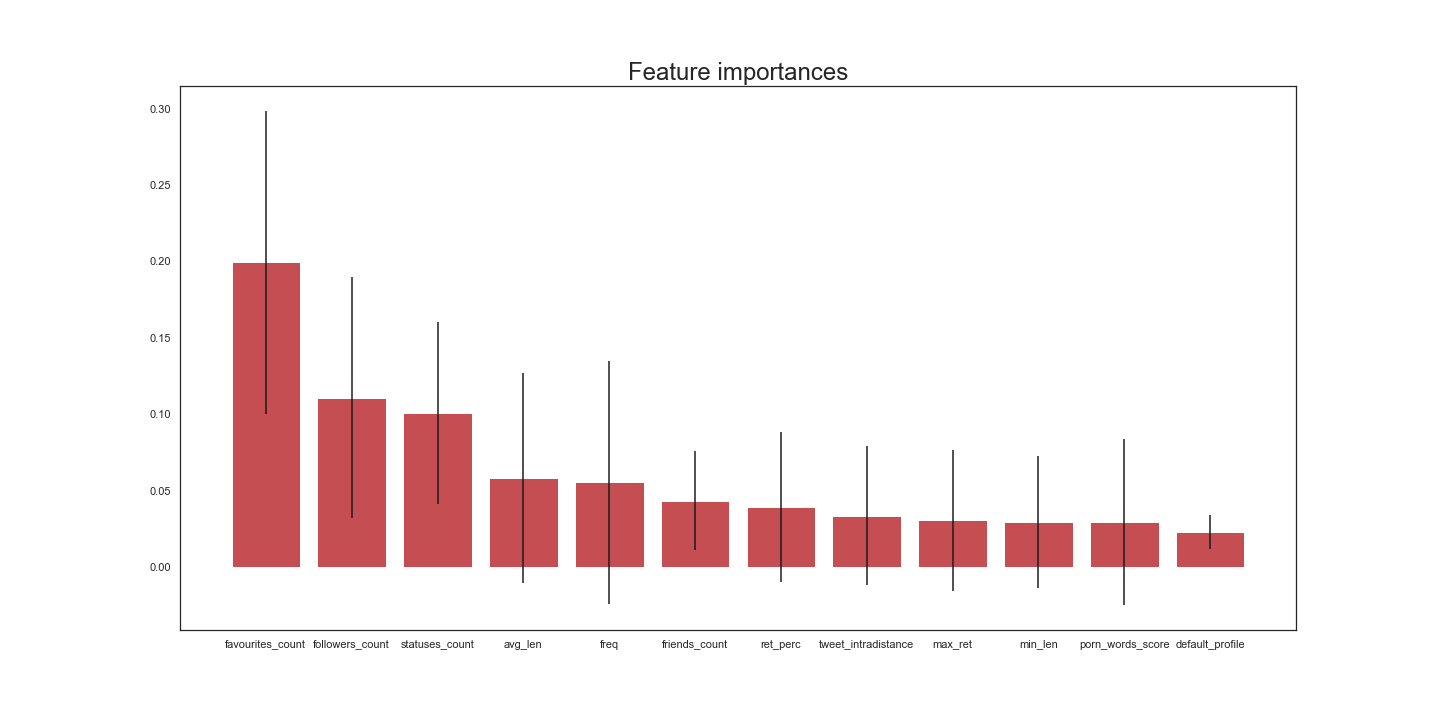
\includegraphics[width=\columnwidth]{chapter5/figure/feature_importances.png}
	\caption{Random Forest feature ranking}
	\label{fig:feature_rank}
\end{figure}

As Figure \ref{fig:feature_rank} shows, we could find some of our crafted features inside this list: lots of tweets descriptive features (\textit{avg\_len, freq, ret\_perc}, etc...), as well as the \textit{tweet\_intradistance} attribute and the \textit{NSFW\_words\_score}.
This picture confirmed us that the idea behind those features was useful.

Since those attributes were thought to belong to different clusters, we decided to try several combinations of those feature clusters, validating the model on them with a crossvalidation. The purpose of this stage was to see if some groups of features were enough to describe the real problem, or if some group would shown up as irrelevant.
To face this evaluation, we performed a light-weighted Grid Search, which is a method that takes desired ranges of hyperparameters and tries all the possible permutations of them, looking for the best combination, in terms of a certain metric.

We are talking about a light-weight version of this tool, because we just went through different numbers of tree estimators in the forest. The different feature groups are not considered as hyperparameters and are not handled by the Scikit-learn implementation of the Grid Search.
We had to manage the different training by our own, looking how the test score would have changed along with the increasing number of estimators and the different set of features.

Grid Search uses crossvalidation to find the better estimators for the models, and this approach was right for our situation.
Due to the multiclass nature and some imbalances with the labels, we decided to follow the F1 score metric to asses the value of our model.

The features were organized in clusters, as described in Chapter \ref{capitolo4}.
We had the user features, the descriptive features, the intrinsic features, the extrinsic and the image features. Then we tried the model with the entire set of 38 attributes.
As shown in Figure \ref{fig:feature_clusters}, the best configuration seems to involve the whole set of features, as it reaches these scores, with 70 estimators: \textit{Precision} = 0.946, \textit{Recall} = 0.945, \textbf{\textit{F1}}= 0.943.
\begin{figure}[htp!]
	\centering
	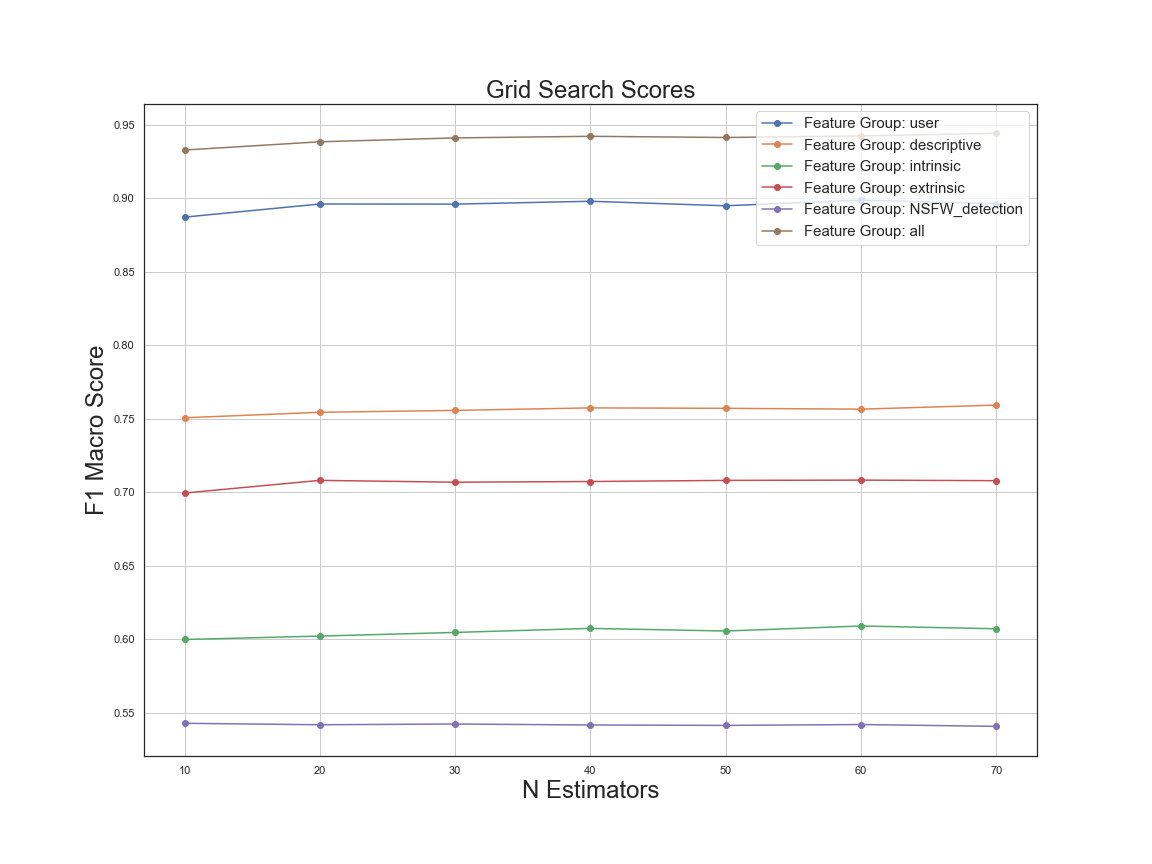
\includegraphics[width=\columnwidth]{chapter5/figure/feature_cluster_f1.png}
	\caption{Performance over different feature clusters}
	\label{fig:feature_clusters}
\end{figure}

The model has been tested with the default value for the maximum depth in the trees, which is set to 'None'. It means that the trees are expanded until every leaf is pure, or all leaves contain one sample.
Tuning the hyperparameters wasn't the goal of this experiment, since its aim was only to find the best configuration of features to fit the model with.

We then continued with a proper Grid Search over the whole number of features.
\begin{figure}[htp!]
	\centering
	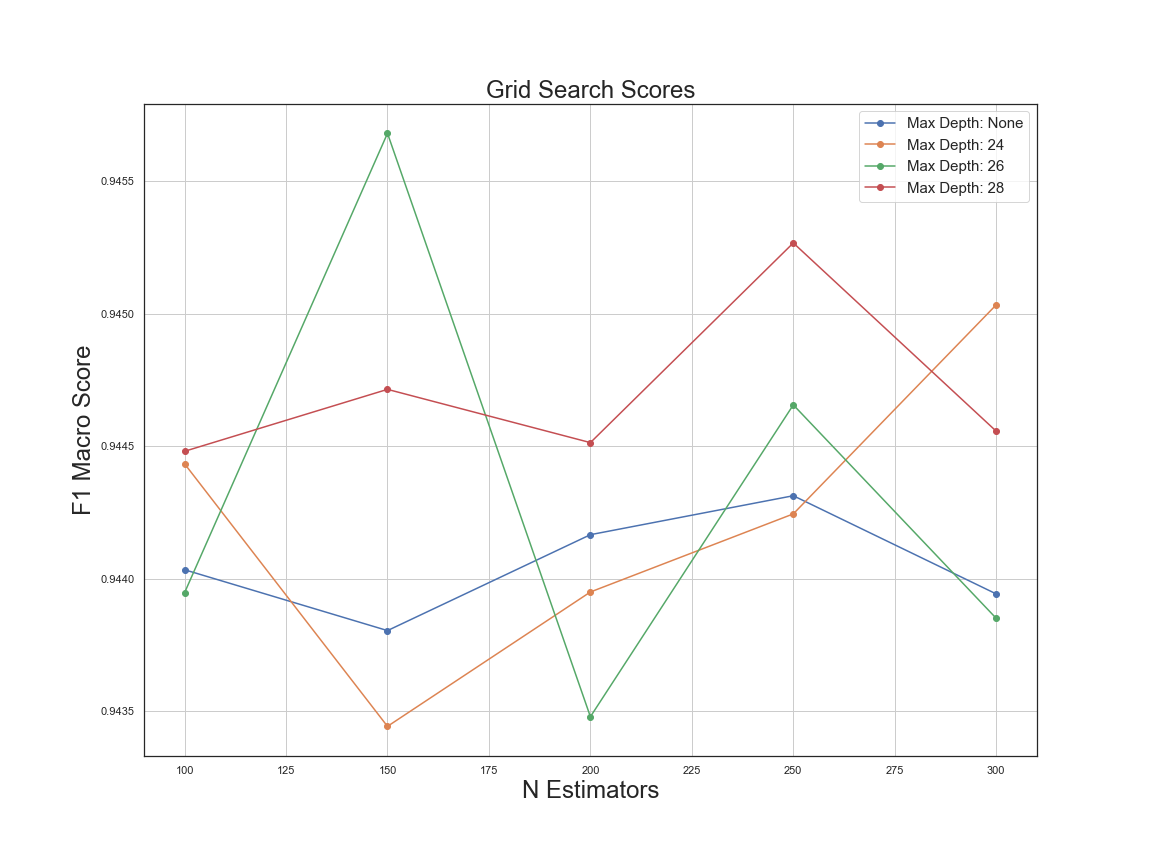
\includegraphics[width=\columnwidth]{chapter5/figure/gini.png}
	\caption{F1 scores with 'Gini' criterion}
	\label{fig:gini}
\end{figure}
\begin{figure}[htp!]
	\centering
	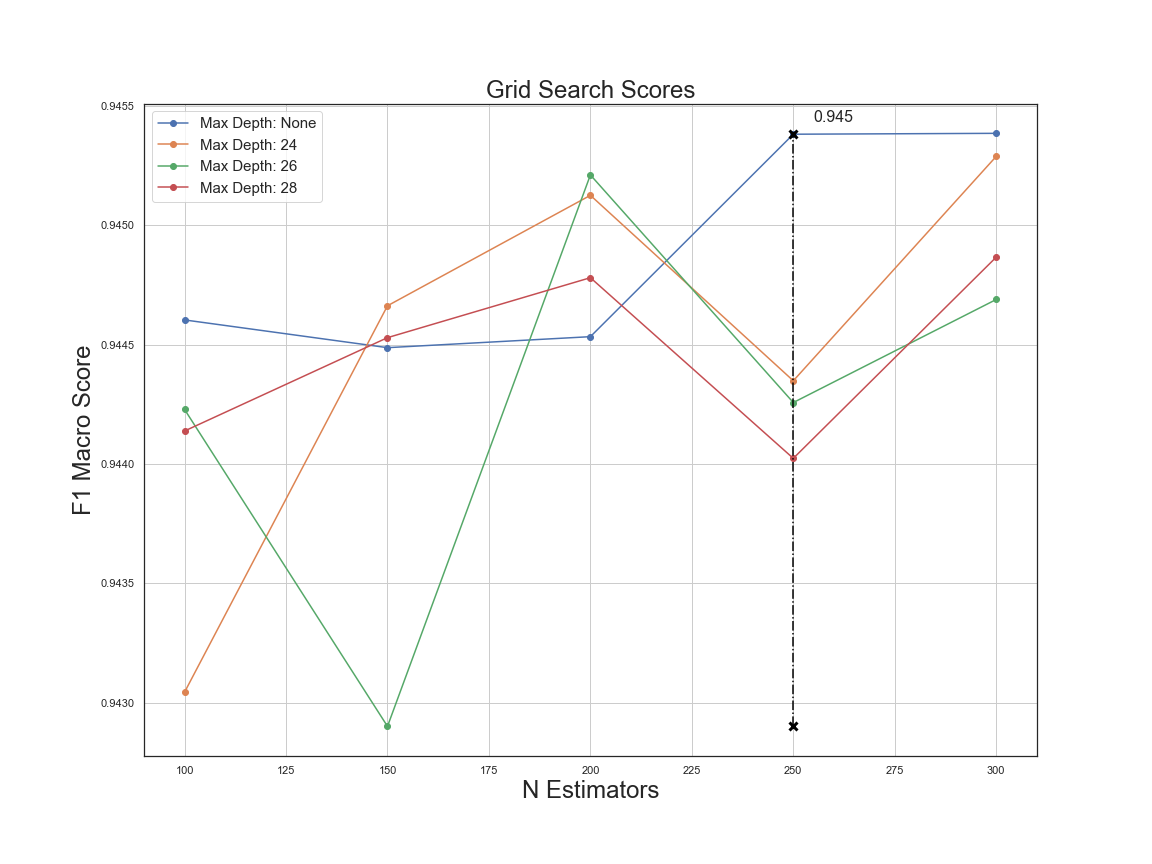
\includegraphics[width=\columnwidth]{chapter5/figure/entropy.png}
	\caption{F1 scores with ''Entropy'' criterion}
	\label{fig:entropy}
\end{figure}

The Figures \ref{fig:gini}, \ref{fig:entropy} show how the average F1 score, measured on 10-fold crossvalidation, changes with the increasing of the number of estimators in the forest.
The different coloured lines represent \textit{max\_depth} hyperparameter.
The first Figure (\ref{fig:gini}) shows the Grid Search results, with the \textit{gini} splitting criterion.
The second one (\ref{fig:entropy}) represent the situation having \textit{entropy} as a splitting choice.
We combined five numbers of estimators (100, 150, 200, 250, 300), together with four different depths of the trees (None, 24, 26, 28) and the two above-mentioned splitting criteria.

We could find a local maximum in \ref{fig:gini}, marked by the green line (\textit{max\_depth = 26}), matching \textit{n\_estimators = 100}. Observing the overall trend for that line, we couldn't rely on that peak, because it seemed to be a lucky hit, due the following lower values accomplished by this configuration. The entropy criterion seemed to be a more stable adjustments of scores, especially with the \textit{None} setting for \textit{max\_depth} hyperparameter.

The highlighted point represent what we pick as our current configuration, and it sees 250 trees, the longest possible depth and the entropy mode for choosing the features on witch separate the trees. 

We decided to stick with the following configuration without continuing with further explorations, because we could observe a flat improvements from 250 to 300 estimators, with that depth.
Furthermore, we were aware that, in the generalization stage, the computation of the image features and the calls to the Twitter APIs would have been taking much more time than the models' predictions, so we decided to have a light model, in order to keep the prediction time fast enough, which is currently measured in 33ms. 

The first algorithm of our solution was completed and ready to be combined with the following two models.

\section{Binary Classifier}
Since our dataset was pretty balanced and we couldn't retrieve much more genuine accounts, we didn't want our instrument to treat this category of users just as one the other bot kinds. It was important to perform a previous filter that was able to give importance to the separation between bots and genuine accounts.

We was inspired by the work made with Botometer\cite{Botometer}, which involved a binary labelled dataset, with bot and genuine accounts.
They built their features, grouped them in six main categories, then they ran a Random Forest algorithm per group.

We already had our feature engineering done, so we decided to test it on this new task.

In order to not to build a poorer version of our multiclass model, we didn't want to use a reduced copy of our dataset, stratifying it by stripping random bots from it. We needed a balanced dataset, with about the same amount of genuines and bots. So, we had to gather more human ids, because if we would have relied on the accounts we already had (3661), we would had disposed on a training set with about 7000 entries, that would have been too small to perform a relevant filter.
\subsection{Dataset}
The dataset we used for this classification was composed by part of our collected records and by some entries from the Carvelee-2011 dataset, which contains 22,223 content polluters and 19,276 legitimate users, both collected through a social honeypot, as described in their paper\cite{Lee11sevenmonths}.
This dataset has been involved to build Botometer as well, but we decided to use it only partially, mixing it with our retrieved accounts.

We setted the APIs to retrieve up tu 6,000 ids for both genuines and bots, from the Carvelee list. The process provided us 5,161 legitimate user ids, and 5,297 general bot ids (without inner classifications), because some accounts have been deleted in time.
Then we added some new records, randomly sampling our data. This led us to reach 7,660 human accounts and 7,795 bots, forming a new dataset of 15,455 entries, with binary target.

The feature vector we used is the same that came out from the feature engineering process\ref{sec:feature_vector}, except for the specific characterizing features, that weren't considered, because crafted for the inner separation among bots. We excluded the image features (\textit{NSWF\_profile} and \textit{NSFW\_avg}) and the extrinsic keywords scores (\textit{NSFW\_words\_score}, \textit{news\_spreaders\_words\_score}, \textit{spam\_bots\_words\_score}, \textit{fake\_followers\_words\_score}, \textit{genuine\_words\_score}).It has been fitted with 32 features.

\subsection{Model}
Since the different purpose of this model, we couldn't rely on the same baselines tested with the multiclass dataset. We wanted to evaluate new raw algorithms for this binary classification.
Another round of crossvalidation, with default settings, was performed on this new dataset, exploiting the binary nature to show the \textit{Area Under the Curve} score (AUC).
Area Under the Curve represents the goodness of a classifier, in terms of the integral of the \textit{Receiver Operating Characteristic} (ROC curve), defined over the variation of a decision treshold.
The motivation behind the adding of this new metric is that we had a balanced binary dataset, and this metric is a good fit for this kind of problem. Moreover, Botmoter claims to have accomplished an AUC of 0.95, on a 10-fold crossvalidation test.

The ROC curve lies in a bi-dimensional space, which has the \textit{True Positive Ratio} ($ TPR =  \frac{TP}{TP+FN}$) on the Y-axis, and the False Positive Ratio ($ FPR =  \frac{FP}{FP+TN}$ ) on the X-axis.

We wanted a term of comparison, so we evaluated this metric even in the baseline stage. Here there are the results of this process:
\begin{itemize}
	\item[\PencilRight] \textit{RandomForestClassifier(n\_estimators = 10, criterion = 'entropy')}\\
	Mean AUC: 0.916\\
	Mean precision: 0.879\\
	Mean recall: 0.793\\
	Mean f1 score: 0.824
	\item[\PencilRight]\textit{LogisticRegression(fit\_intercept=True, max\_iter=100, penalty='l2')}\\
	Mean AUC: 0.792\\
	Mean precision: 0.694\\
	Mean recall: 0.759\\
	Mean f1 score: 0.723
	\item[\PencilRight]\textit{KNeighborsClassifier(n\_neighbors=10)}\\
	Mean AUC: 0.835\\
	Mean precision: 0.779\\
	Mean recall: 0.750\\
	Mean f1 score: 0.760
	\item[\PencilRight]\textit{SVC(kernel='rbf', decision\_function\_shape='ovo')}\\
	Mean AUC: 0.583\\
	Mean precision: 0.620\\
	Mean recall: 0.364\\
	Mean f1 score: 0.095
\end{itemize}
Once again, Random Forest won the comparison with the other baselines.
We decided to let it perform this job and try to improve its AUC score, keeping one eye on the overall score too.

The algorithm has had its parameters tuned during the validation phase.
We decided to stick with 10-fold crossvalidation, as it was done for the baselines.

After several Grid Search runs, the last round computed had this hyperparameters to combine together:
\begin{itemize}
	\item[\PencilRight] \textit{n\_estimators} = [100, 115, 130, 150, 175, 200]
	\item[\PencilRight]\textit{max\_depth} = [None, 26, 28]
	\item[\PencilRight]\textit{criterion} = 'entropy'
\end{itemize}
\begin{figure}[htp!]
	\centering
	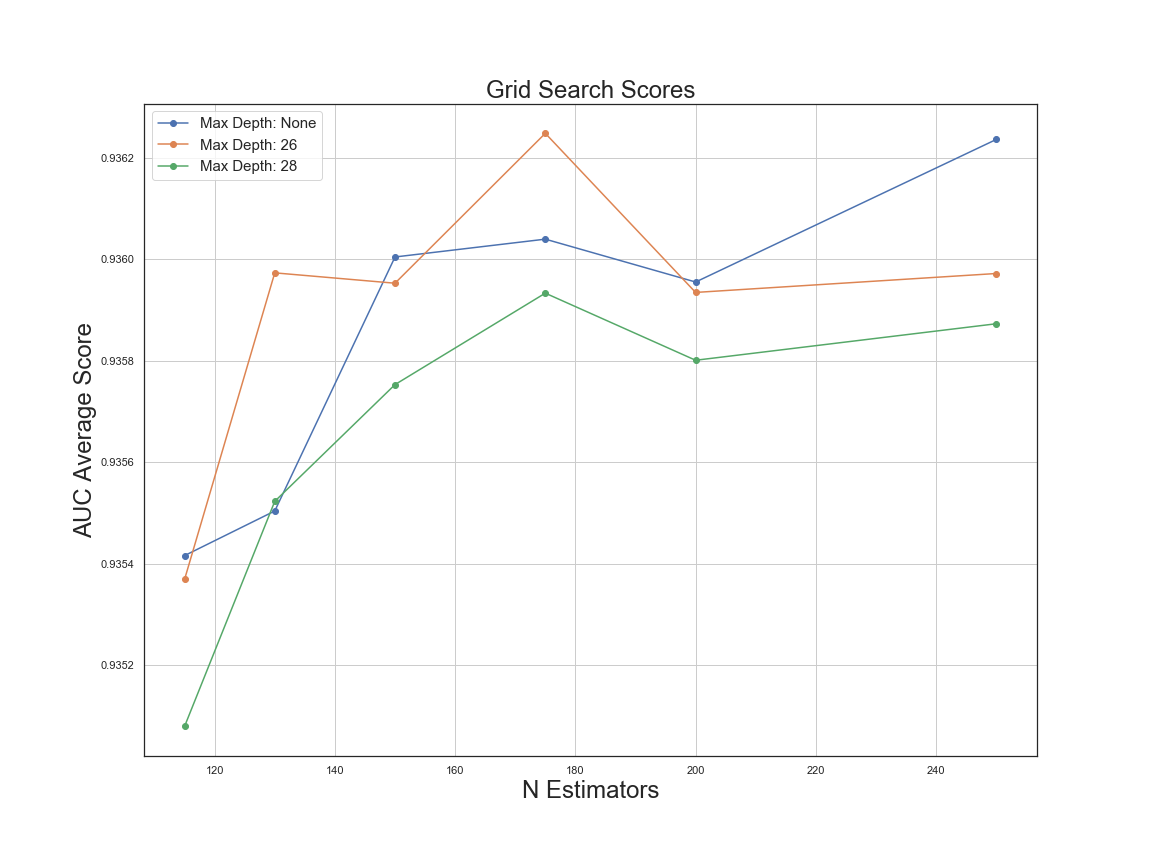
\includegraphics[width=\columnwidth]{chapter5/figure/gridSearch.png}
	\caption{Grid search results}
	\label{fig:grid_search}
\end{figure}
\begin{figure}[htp!]
	\centering
	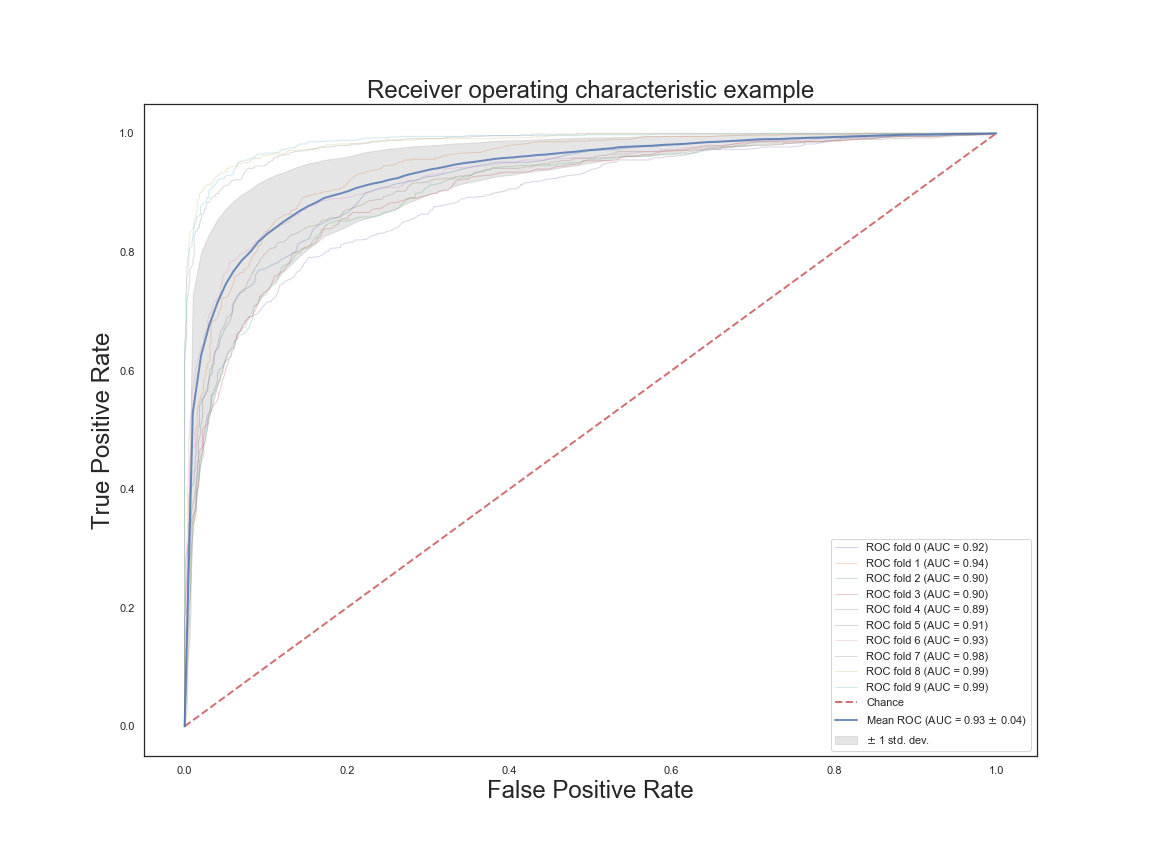
\includegraphics[width=\columnwidth]{chapter5/figure/auc.png}
	\caption{ROC curve}
	\label{fig:auc}
\end{figure}
As we can see in Figure \ref{fig:grid_search}, the AUC is increasing with the number of the estimators in the forest. We decided t stop at 250, which corresponds to the highest AUC score, with a low risk to perform overfitting.

The AUC obtained with this arrangement is equal to 0.936, as shown in Figure \ref{fig:auc}, which is a positive accomplishment, considering that it will be used only as support for the identification of humans among bots, but we didn't crafted specific features as the ones involved in the Botmoter project and we didn't have the same amount of data neither.

The final model has been fitted with the hole data, with this settings: \textit{ n\_estimators} = 250, \textit{max\_depth} = None and \textit{criterion} = 'entropy'.
The max\_depth parameters states how deep the tree should be expanded. When set to \textit{None}, the algorithms tries to expand them until every leaf if pure.
We were looking for this approach, because we wanted this filter classifier to be ensure the hardest classifications possible, among a soft classification system. We wanted some loose detections, when there were no certainties. But we wanted the prediction to be as sure as possible, when no uncertainties were met. 

Once we fitted the model, it was ready to be the second element entering in our solution pool.

\section{Text classifier}
\section{Stacking meta-classifier}
We had three models, each with different purposes, but they had to cooperate for the bots' behaviour identification.
The initial idea was to use only the multiclass Random Forest to classify the bot categories, using the other two models as meta-models to build extra features with their outcome.
Those features would have had the dataset enhanced, but their meaning would have been bounded to the multiclass classifier limits.
We wanted to give the right importance to each model, hoping they would help each other to better distinguish the patterns end to better model the real problem.

We thought about several methods to exploit their strengths and combine them.
The first idea was to build a pipeline with weights for each classifier. The binary Random Forest would had been the first filter between humans and bots. Following this lead, the multiclass and the text classifiers would have been weighted in order to assign the final label.

This approach would have been less empirical then other tools we could dispose. We decided to rely on different methods to blend the outcomes of our three algorithms. In particular, we thought about a genetic approach and a stacking ensemble with a meta-classifier. 
We wanted to evaluate the performance obtained by these methods and chose the one that fitted our need.

Both the genetic and the meta-model were trained with holdout technique, splitting the whole dataset into training and test sets. The 80\% of the samples ended up into the training set, the 20\% in the validation set.
We had a training set for the ensemble models that contains 5022 entries.
The data that fed the stacking methods were the predictions of the tree classifiers, over the validation set.
In order to make those prediction without cheating, we couldn't use the models that were already fitted with the hole data. We had to retrain them with the 80\% of the records. 
We didn't perform further Grid Search to find the best hyperparameters in this stage, because the final script that we were going to assemble was taking into account the entire dataset to train the models. Furthermore, this small variation, in terms of amount of training data, wouldn't had led us into a misinterpretation of the problem, if we had kept the same hyperparameters found earlier.
We decided to stick with the configurations already found and to train the model with fewer data.

Once the model were fitted, we used the \textit{predict\_proba()} method of the Scikit-learn implementations of the classifiers, in order to retrieve "soft classifications".
We didn't want our model to assign a strict label to an unseen sample, indeed, we were interested in the percentage of categories membership.
The predict\_proba() method computes the probability, for a sample, to belong to the highlighted target, by considering the impurity of the leaves inside the forest.
We used this method to construct the output vectors needed to train the stacking models.

In order to combine the outputs of three classifiers properly, we had to homologate them.
With the multiclass and the text models there weren't issues, since their outcomes are stored into vectors with five elements, containing probability values, one for each category.
The case to handle was the binary one, because the output of that Random Forest was represented by a 2-sized vector (the bot probability and the genuine one).
We extended the array adding three more cells. Then we took the bot probability and spread it on the four cells that didn't mark the genuine probability.
The reason behind that is that our binary classifier didn't take care about the inner separation in bot behaviours. It was uncertain about the belonging category, it just used to recognize bots, so each non-human category should had been assigned the same coefficient, and their sum must had match the original probability to be detected as a bot.
For instance, if the binary classifies detects an account with 80\% chance to be a bot and 20\% to be genuine, it will result in this final outcome vector:
\begin{center}
	\begin{tabular}{ccccc}
		\\Bot&Genuine\\
		\hline
		0.8&0.2\\
		\hline\\
	\end{tabular}\\
Original binary output
\end{center}
	
\begin{center}
	\begin{tabular}{ccccc}
		\\NSFW&News-Spreader&Spam-Bot&Fake-Follower&Genuine\\
		\hline
		0.2&0.2&0.2&0.2&0.2\\
		\hline\\
	\end{tabular}\\
Adapted multiclass output
\end{center}

Each sample of this new dataset contains 15 elements, 5 soft predictions (one for each category) for each classifier (binary, multiclass, text-based).
\begin{center}
	\begin{tabular}{@{}c|c|c|c|c|c|c|c|c|c|c|c|c|c|c@{}}
		\multicolumn{15}{c}{New sample} \\
		\hline
		\multicolumn{5}{c|}{Binary probability} & 
		\multicolumn{5}{c|}{Text-based probability} & 
		\multicolumn{5}{c}{Multiclass probability}\\
		\hline
		p\textsubscript{0} &
		p\textsubscript{1} &
		p\textsubscript{2} &
		p\textsubscript{3} &
		p\textsubscript{4} &
		p\textsubscript{5} &
		p\textsubscript{6} &
		p\textsubscript{7} &
		p\textsubscript{8} &
		p\textsubscript{9} &
		p\textsubscript{10} &
		p\textsubscript{11} &
		p\textsubscript{12} &
		p\textsubscript{13} &
		p\textsubscript{14}\\
		\hline
	\end{tabular}
\end{center}
A new training set was born and it was built with the soft classifications of the models in the pool, over the validation set. It was ready to proceed and to serve the ensemble models.\\

\begin{figure}[htp!]
	\centering
	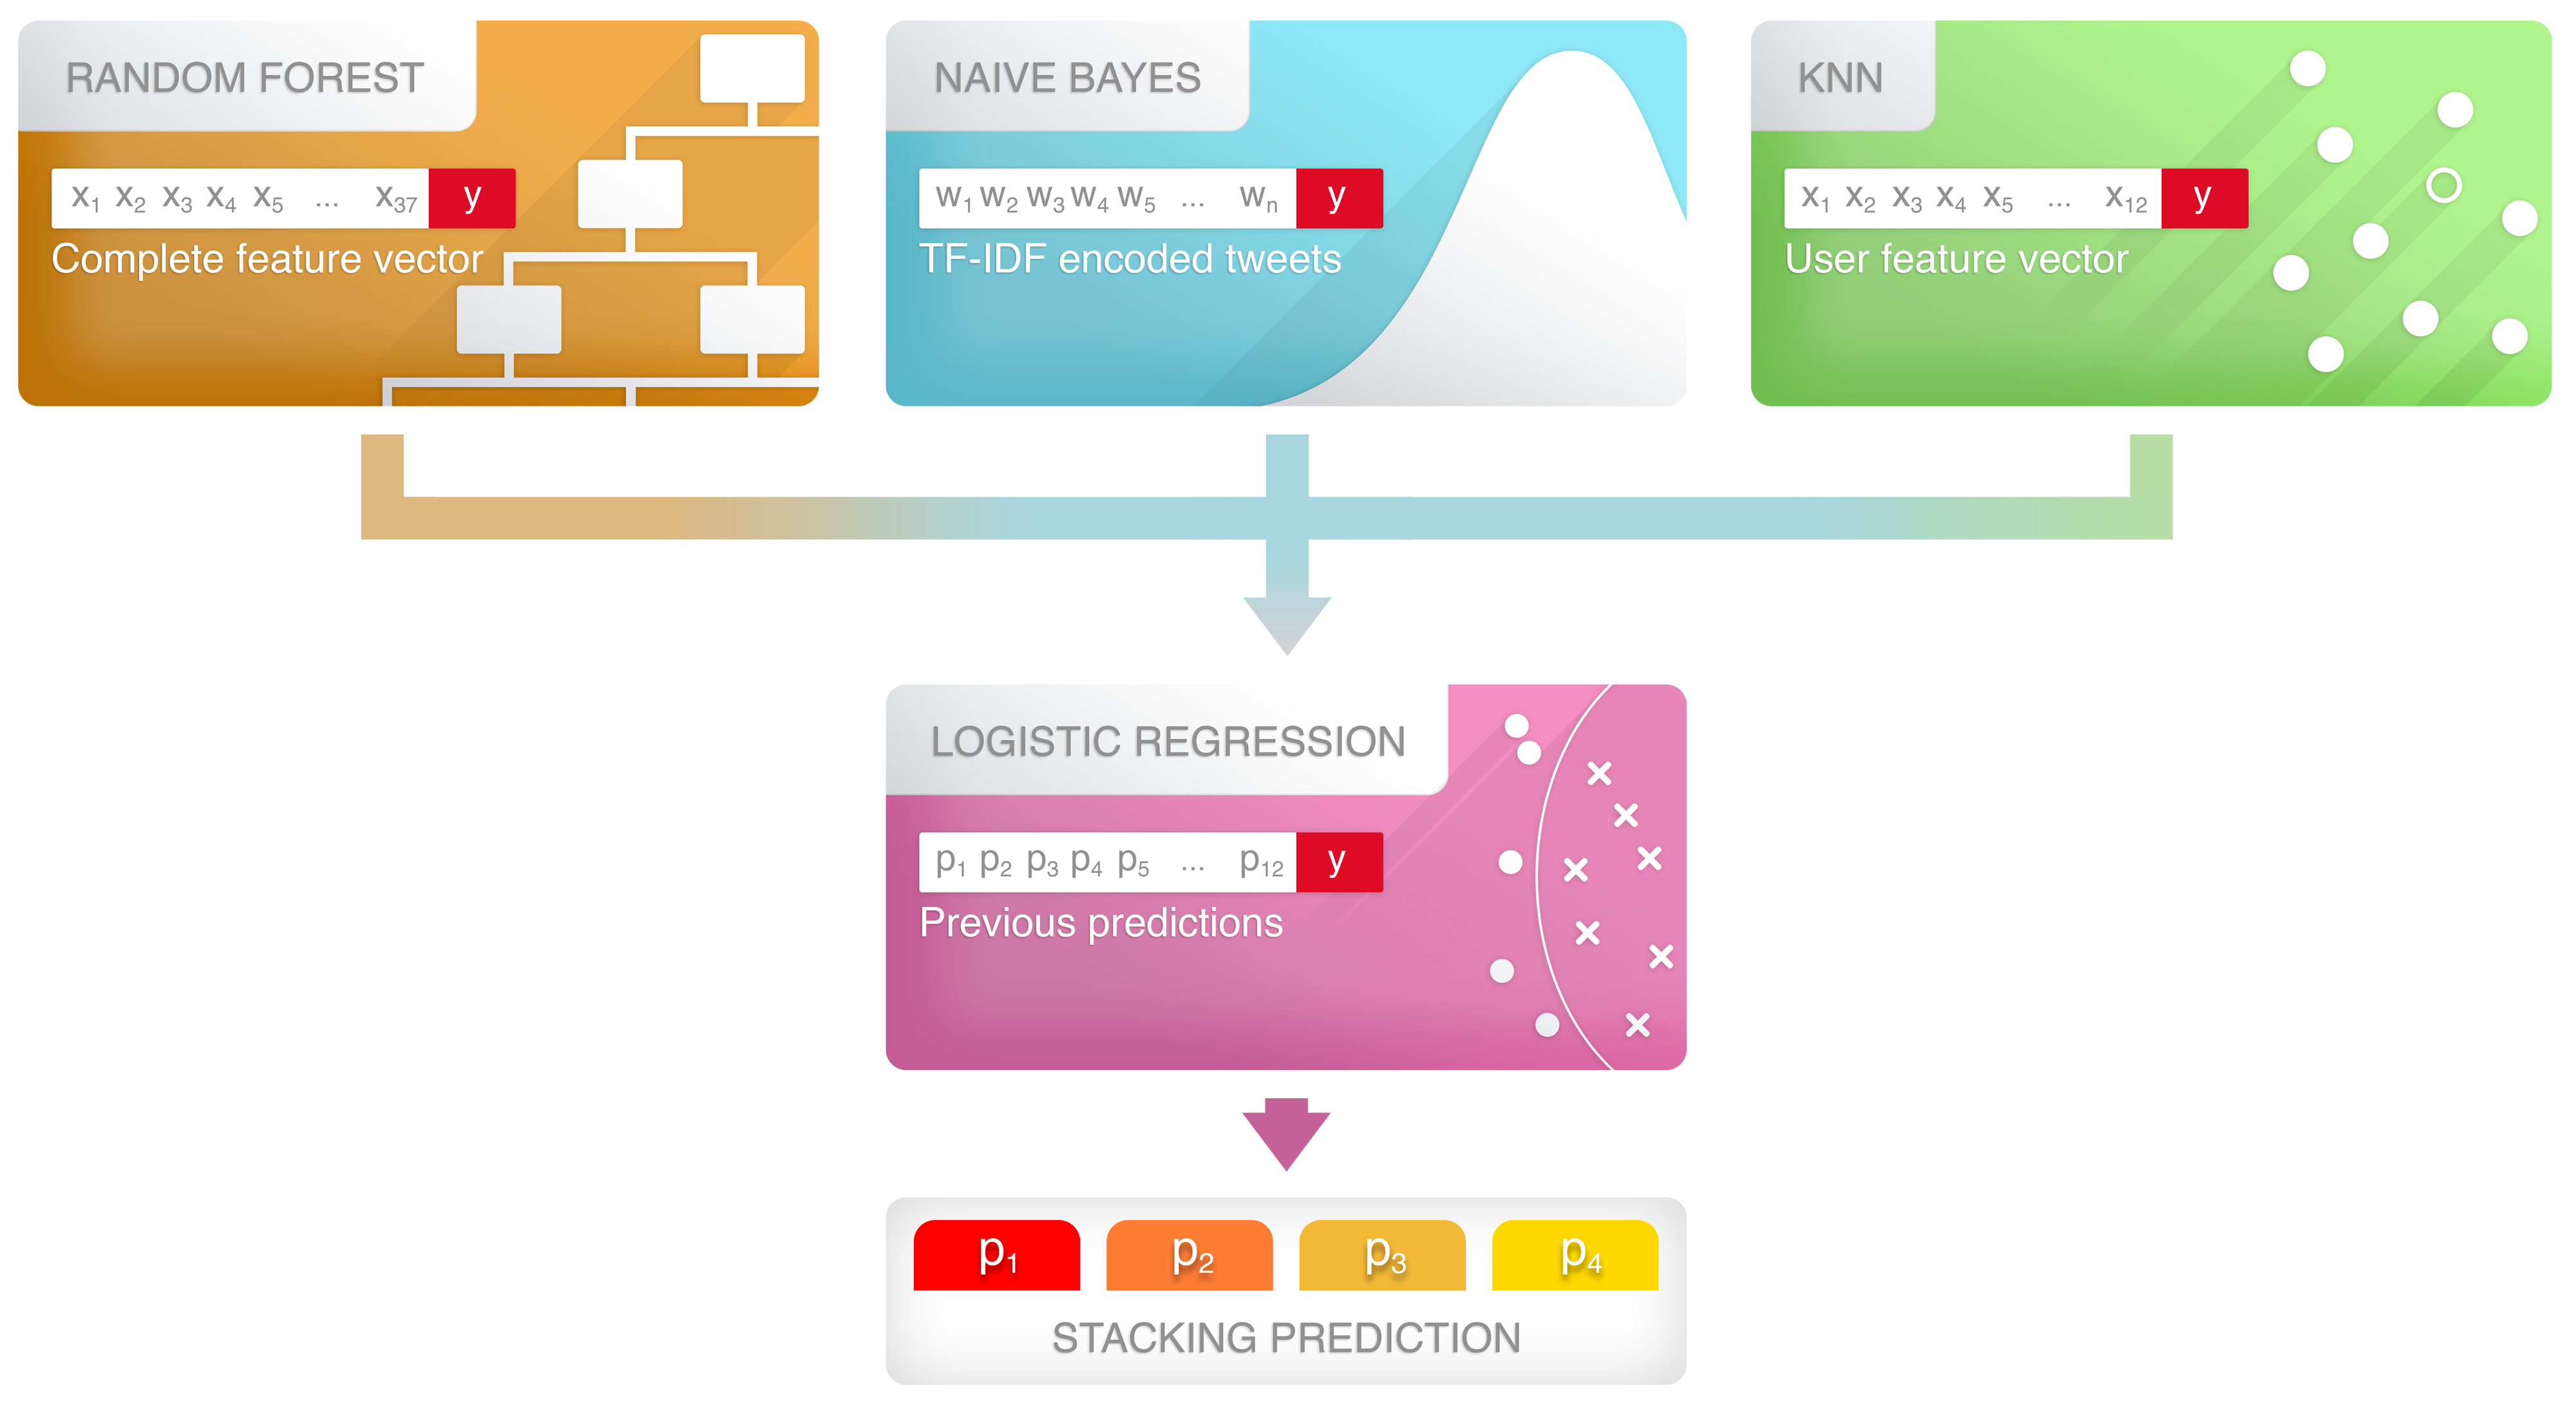
\includegraphics[width=\columnwidth]{chapter5/figure/stacking.png}
	\caption{Training pipeline of theNodv stacking ensemble}
	\label{fig:stacking_pipeline}
\end{figure}
The pipeline for perform the training of the ensemble models is resumed in Figure \ref{fig:stacking_pipeline}.

After several parallel attempts were done, the blending system was built with the meta-classifier.

\subsection{Genetic algorithm}
This approach started as a side way, when we were already testing the stacking ensemble.

The idea behind genetic programming, is to emulate the natural species evolution, by encoding the the \textit{chromosomes} in the process with data structures.
The chromosomes represent the possible solutions for the problem and they have to "evolve", in order to get fitter and fitter for the goal.
Several operators must be determined to perform this evolution.
Once a first \textit{generation} of feasible chromosomes has been formed, they have to be evaluate according to a \textit{fitness function}, which asses how well a chromosome faces the problem.
The best portion of chromosomes are picked to be part of the next generation, and this is called \textit{elitism}. The solutions left are given a probabilities to join the elite ones, in order to form a new generation with about the same size as the previous. This step is called \textit{selection}.
The chromosomes picked in the selection stage are assigned a high \textit{crossover} probability.
The crossover operator handles the "born" of new chromosomes, mixing parents alleles in a certain way. The mixing method is highly correlated to the chosen encoding strategy.
Each newborn is give a low probability to undergo a mutation. This step often seems useless, but it's pretty important, in order to explore a higher spectrum of solutions, which couldn't be expanded by the mating operators only.
After the new population has been accepted, it is ready to be validated through the previously define fitness function.
The loop holds, until a solution is found, or, like in our case, the process sticks to a local or global maximum.

\subsubsection{Genetic operators}

We setted the genetic algorithm with the support of the Deap library for Python, setting these operators:
\begin{itemize}
	\item[\PencilRight]\textit{Encoding}: each chromosomes represented a weighting vector for the outcome of our three classifiers. Each allele of the chromosome was float valued, with numbers between 0 and 5, generated randomly, with a uniform distribution. We started with normalized weights, but the spectrum of the solution explored was way too poor to fit the needs.
	This range was given after observing the weights that the Logistic Regression model were assigning to the inputs received, that was wider and involved even negative values.
	We randomly generated 200 chromosomes for the initial population, with this form.
\end{itemize}
	\begin{center}
		\begin{tabular}{@{}c|c|c|c|c|c|c|c|c|c|c|c|c|c|c@{}}
			\multicolumn{15}{c}{Chromosome} \\
			\hline
			\multicolumn{5}{c|}{Binary Weights} & 
			\multicolumn{5}{c|}{Text-based Weights} & 
			\multicolumn{5}{c}{Multiclass Weights}\\
			\hline
			w\textsubscript{0} &
			w\textsubscript{1} &
			w\textsubscript{2} &
			w\textsubscript{3} &
			w\textsubscript{4} &
			w\textsubscript{5} &
			w\textsubscript{6} &
			w\textsubscript{7} &
			w\textsubscript{8} &
			w\textsubscript{9} &
			w\textsubscript{10} &
			w\textsubscript{11} &
			w\textsubscript{12} &
			w\textsubscript{13} &
			w\textsubscript{14}\\
			\hline
		\end{tabular}\\
	\end{center}
\begin{itemize}
	\item[\PencilRight]\textit{Fitness evaluation}: the fitness function that assessed the value of the solutions was somehow similar to the one used in the other stacking method.
	We applied the weights of our chromosomes to the samples in our dataset.
	
	For each sample, we made pairwise additions, among the outputs of different classifiers, multiplied by the chromosome's weights, for the same category:
	\begin{center}
		\begin{tabular}{@{}c@{}}
			
			\multicolumn{1}{c}{Binary Components}\\
			\hline
			\multicolumn{1}{c}{p\textsubscript{0} * w\textsubscript{0} ... p\textsubscript{4} * w\textsubscript{4}}\\
			\hline\\
			\multicolumn{1}{c}{+}\\
			
			\\\multicolumn{1}{c}{Text-based Components}\\
			\hline
			\multicolumn{1}{c}{p\textsubscript{0} * w\textsubscript{0} ... p\textsubscript{4} * w\textsubscript{4}}\\
			\hline\\
			\multicolumn{1}{c}{+}\\
			
			\\\multicolumn{1}{c}{Multiclass Components}\\
			\hline
			\multicolumn{1}{c}{p\textsubscript{0} * w\textsubscript{0} ... p\textsubscript{4} * w\textsubscript{4}}\\
			\hline\\
			\multicolumn{1}{c}{=}\\
			
			\\\multicolumn{1}{c}{Resulting Prediction}\\
			\hline
			\multicolumn{1}{c}{\textbf{p\textsubscript{0}} \textbf{p\textsubscript{1}} \textbf{p\textsubscript{2}} \textbf{p\textsubscript{3}} \textbf{p\textsubscript{4}}}\\
			\hline\\
		\end{tabular}
	\end{center}
	
	In order to stick to the probabilities nature, the computed prediction had been normalized.
	
	That prediction has been compared with the known real target for the examined sample.
	Since the targets of our dataset aren't soft valued, we took the maximum probability of the computed prediction to make the comparison with the actual class.
	Our fitness function aims to favourite those solutions which maximizes the F1 macro score, as it has been for the validation of the classifiers, until this stage.
	
	During this process, the problem we had to face was that we wanted to produce soft classifications, because we knew that our collected data presents similar patterns within the same categories. This means that the algorithms easily classify our test set, because of the distinctive traits found for each target. In order to mitigate the real test error, over unseen samples, we wanted the prediction to be as smooth as possible, without confusing the F1 score interpretation. In addition, the multiclass Random Forest was setted with the maximum depth possible for its estimators, that implies a drastic reduction of impure leaves, leading to hard classifications.
	
	We faced the problem involving a smoothing factor to our fitness function.\\
	When computing a sample, we populated a Confusion Matrix of the prediction, using the above-mentioned method to match predicted and actual classes. The matrix helped us computing the F1 macro score easily. At the same time, we counted every hard classification, marking as 'hard' every computed prediction that contained a probability greater or equal to \textbf{0.8}, among its five stored values.
	This count was used as a penalty, it has been averaged for the number of samples, and then subtracted to the computed F1 score of that chromosome. In order to privilege the maximization of the F1 factor, instead of the minimization of the penalty, the final fitness function assigned this score to each chromosome:
	\[ Fitness = 3 \times F1\_score - Penalty \]
	This way to operate didn't affect the overall F1 of the sample, since penalizing hard classifications didn't discourage the system to look for values high enough to have a dominant category in the prediction.
	
	Once every chromosome has been evaluated, they could proceed to the next steps of the algorithm.
	
	\item[\PencilRight]\textit{Selection}: the selection phase handles the choice over which chromosomes pick for mating. Several pre-implemented methods are available, but we used the tournament method. It works selecting the size \textit{K} of the tournament, which we chose to be 3. Then, it randomly selects \textit{K} (3) chromosomes from the population and places it inside a pool. Then it compares their fitness. The chromosome with the best fitness has probability \textit{p} (the crossover probability) to be selected for mating. The second has $ p*(1-p) $ chance to get selected, the third $ p*((1-p)^{2}) $.
	\item[\PencilRight]\textit{Crossover}: The crossover probability has been setted to 95\%.
	The crossover operator wasn't something already implemented by the library, as for the fitness function. Our operator used to produce two brand new chromosomes for the next generations.
	The first child is the unweighted mean of its parents:
	\[ [x_{0}, x_{1}, ... x_{14}] \oplus [y_{0}, y_{1}, ... y_{14}] = [\frac{x_{0}+y_{0}}{2}, \frac{x_{1}+y_{1}}{2}, ... \frac{x_{14}+y_{14}}{2}]\]
	The second child is the weighted mean of its parents, computing the weights with respect to the fitness of the two mating chromosomes:
	\[ f_{x} = \frac{fitness_{x}}{fitness_{x}+fitness_{y}} \]
	\[ f_{y} = \frac{fitness_{y}}{fitness_{x}+fitness_{y}} \]
		\[ [x_{0}, x_{1}, ..., x_{14}] \oplus [y_{0}, y_{1}, ..., y_{14}] = [x_{0}*f_{x}+y_{0}*f_{y}, ... x_{14}*f_{x}+y_{14}*f_{y} ]\]
		
	The retrieved children used to be part of the upcoming generation.
	\item[\PencilRight]\textit{Elitism}: This part was necessary, in order to not lose the best solutions found so far. It is a sort of insurance, which guarantees to keep, at least, the best situation until this stage, and to let it take part of the next generations of solution. We preserved our three best chromosomes for each generations and move them to the next stages.
	\item[\PencilRight]\textit{Mutation}: The mutation probability is generally setted to low values, like what happens in nature. It represent the error in DNA replications from the parents and it shouldn't reach the 1\% of probability to occur.
	Although, we wanted to force some mutation, because, as said before, we needed a wider space of solutions and the elitism helped us in containing the damages of such mutations. In the worst cases, all the chromosomes have had been damaged and resulted as useless, but the elitism had preserved the best ones and kept it untouched. So we imposed a 45\% of mutation probability, for each newborn solutions, before entering the pool.
	
	Our mutation operator was a decoration of the value changing method already implemented: we randomly used to pick three elements from the chromosome and set them to zero.
\end{itemize}

\subsubsection{Results}
After several runs of the genetic program, with boosted starts (the best solutions found at the previous run were placed inside the first generations of the following runs), we stuck in a maximum of the F1 score.
In the last run, from the 5\textsubscript{th} generation there was no improvements in the fitness of the best solution. We selected the fittest chromosome, whose scores were:
\begin{itemize}
	\item[\PencilRight] \textit{Weights}:

	\begin{center}
		\begin{tabular}{@{}c|c|c|c|c@{}}
			\hline\hline
			\multicolumn{5}{c}{\textbf{Binary Weights}}\\
			\hline
			\multicolumn{1}{c|}{0.0}&
			\multicolumn{1}{c|}{0.234}&
			\multicolumn{1}{c|}{0.0}&
			\multicolumn{1}{c|}{4.145}&
			\multicolumn{1}{c}{2.668}\\
			\hline
			\multicolumn{5}{c}{\textbf{Text-based Weights}}\\
			\hline
			\multicolumn{1}{c|}{4.867}&
			\multicolumn{1}{c|}{2.808}&
			\multicolumn{1}{c|}{4.680}&
			\multicolumn{1}{c|}{2.800}&
			\multicolumn{1}{c}{2.325}\\
			\hline
			\multicolumn{5}{c}{\textbf{Multiclass Weights}}\\
			\hline
			\multicolumn{1}{c|}{4.462}&
			\multicolumn{1}{c|}{2.129}&
			\multicolumn{1}{c|}{2.162}&
			\multicolumn{1}{c|}{2.317}&
			\multicolumn{1}{c}{0.163}\\
			\hline\hline
		\end{tabular}
	\end{center}
	\item[\PencilRight] \textit{Fitness}: 2.184
	\item[\PencilRight] \textit{F1 score}: 0.964
	\item[\PencilRight] \textit{Percentage of hard classifications}: 70.8\%
\end{itemize}
The solution found didn't take into account the first and the third element of the input, which correspond with the outcome of the binary classifier, for both the NSFW and the Spam-Bot categories. It seemed legit, because the main difference between that model and the multiclass classifier, except the binary task, is the lacking of the NSFW specific features. It makes sense that this model wasn't able to contribute to the separation between those kinds of bot.
That feature vector should had been involved in the final model, simply as a weight for the weighted mean of the probability of each classifier, for each sample to predict over.

Although the result seemed promising, we knew that a "simple" weighted mean of the outcomes of the classifiers weren't enough to describe the problem. The risk to have performed overfitting over our data was high.

We decided to test this final weighting vector with new unseen samples, selected manually for the purpose.
The comparison with picked samples didn't match the expectations given by the metric evaluation, so we tried a different and more sophisticated stacking method.

\subsection{Logistic Regression}
The reason behind the choice of a meta-classifier is that we wanted a more complex way to perform inner weighting of the outcomes that we had from other models.
A simple weighted mean wasn't enough for this purpose. Furthermore, implementing a logistic-like loss to evaluate the fitness of a genetic algorithm would have mean to apply the Logistic Regression training model, without performing gradient descent, but with a genetic approach. It would have been just unnecessary and computationally expensive.
Thus, we discarded the idea of using the genetic programming to emulate a Logistic model, even if the smoothing factor used for that try was a good insight for our task.
In order to mitigate the lacking of soft classifications, we chose to rely on the regularization factors that belong to the training algorithm of the Logistic Regression.
This kind of models is often involved in stacking other classifiers, with a binary purpose.

\subsubsection{Dataset}
The same training set has been used for train both the Genetic and Logistic models.
Since we were managing a multilabel datasets, we knew that the ensemble meta-model would had been adapted to this job. The most common tool used for stacking purposes is the Logistic Regression, which performs well on binary separations. We decided to test this model on a multinomial approach, with a softmax activation function, instead of trying the already visited One-vs-Rest method.

\subsubsection{Comparison with Random Forest}
We didn't wanted to blindly select this model over some others tool, especially over Random Forest, which proved us to perform well in multiclass classifications.
Thus, we tested these two algorithms with the new dataset.
We ran some default configurations of the models, in order to have a raw comparison to trace a line between them.

\begin{figure}{htp!}
	\begin{multicols}{2}
		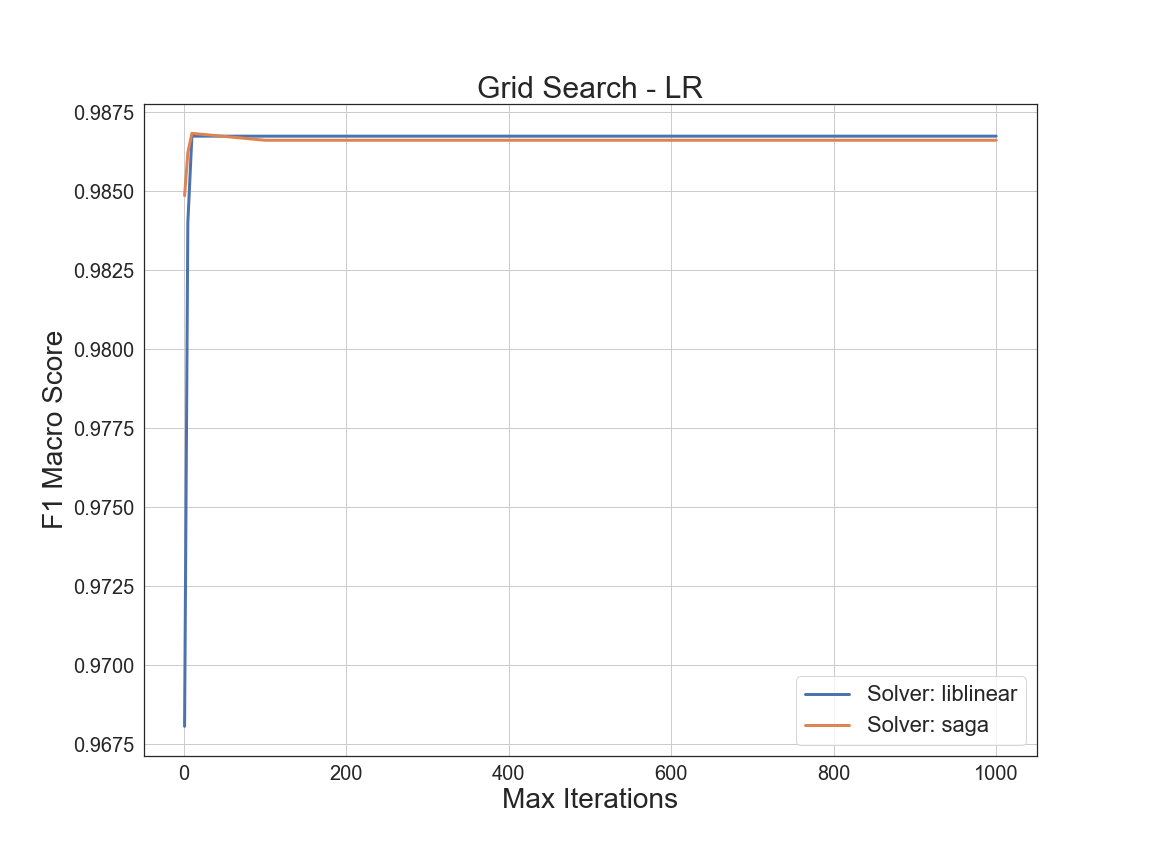
\includegraphics[width=\linewidth]{chapter5/figure/logreg_default.png}\par 
		\caption{LogReg with raw settings}
		\label{fig:lr_def}
		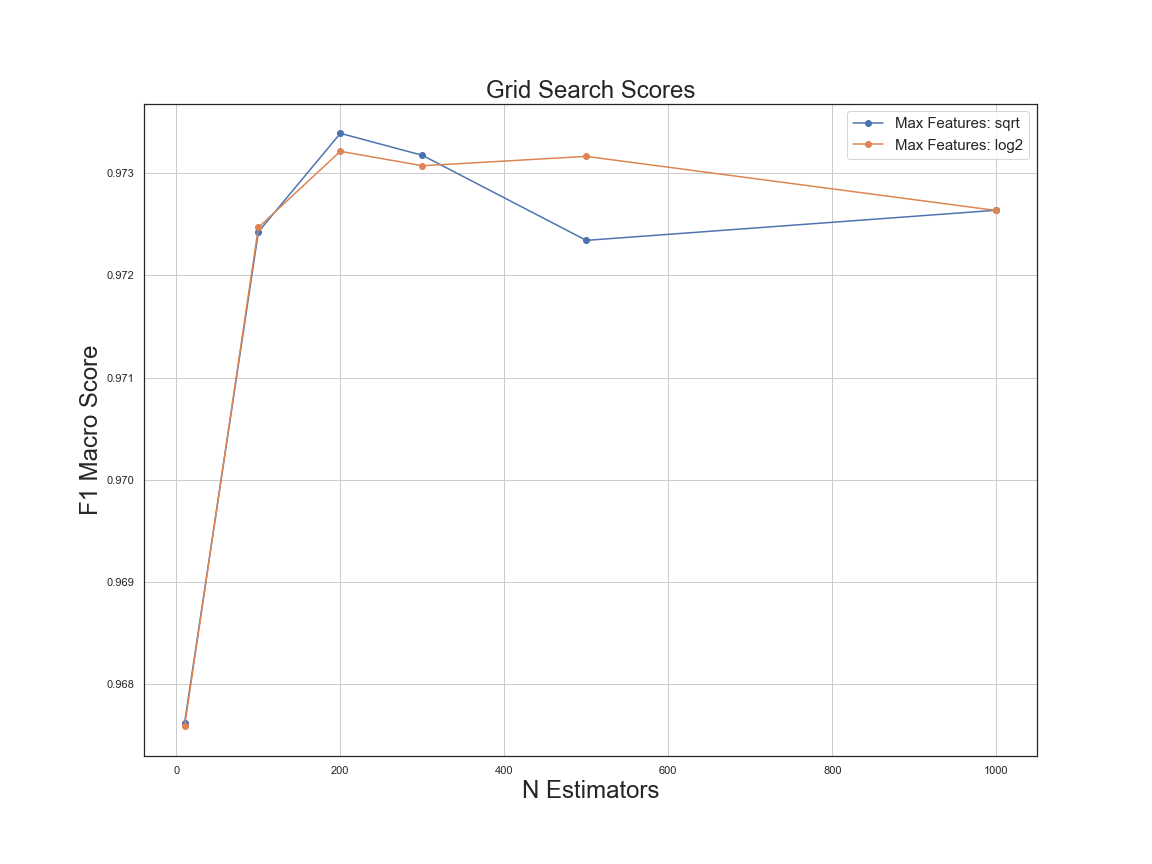
\includegraphics[width=\linewidth]{chapter5/figure/random_forest_default.png}\par 
		\caption{Random Forest with raw settings}
		\label{fig:rf_def}
	\end{multicols}
	\caption{Stacking models comparison}
\end{figure}

Figure \ref{fig:lr_def} shows the early convergence of the Logistic model's F1 score, with low maximum iterations. The model has been tested with Lasso penalty and two different solvers, but the results, over the increasing of the training epochs, are way similar.
The Random Forest, as shown in Figure \ref{fig:rf_def}, needs lot of estimators to top the performance of the Logistic Regression. It was tested over the number of features to consider for the splits ($ \log(|features|) $ and $ \sqrt{|features|} $), along with an increasing number of trees.

We preferred the lighter Logistic model over the Forest ensemble, for performance matters and prediction time: Logistic predictions take 0.6ms in average, in comparison with Random Forest with those settings, which averages 100ms to provide an outcome over a single sample.

\subsubsection{Hyperparameters tuning}
We tried two regularization terms for the Logistic model and several numbers of maximum iterations for the training algorithms.
The regularization terms are parameters computed in addition with the minimization of the characteristic loss function. Their purpose is to avoid the weights to explode and the model to become more sensitive to noisy data. In other words, they are involved to prevent overfitting.
The idea is that the loss function, gets modified as follows
\[ \mathbf{L(w)} = L_{D}(w) + \lambda L_{W}(w)\]
Where $ L_{D}(w)  $ represent the error on the data and $ L_{W}(w)  $ is the term representing the model complexity. In general, smoother weights implies lower model complexity. The lighter the complexity, the lower the variance of the model and the risk perform overfitting.
The parameter $ \mathit{\lambda} $ has to be tuned with a validation method.

The penalties that we explored were:
\begin{itemize}
	\item[\PencilRight] \textit{Lasso (L\textsubscript{1})}:
	\[ \mathbf{L_{1}(w) }= \frac{\lambda}{2} ||\mathbf{w}||_{1} \]
	where $ ||\mathbf{w}||_{1} = \sum_{i=1}^{N}|w_{i}| $
		
	This regularization function is non-linear and doesn't provide a closed-form solution. It tends to cut out some features from the model, yielding to sparse and lighter model. It can be seen as an implicit way to apply features selection.
	
	\item[\PencilRight] \textit{Ridge (L\textsubscript{2})}:
	\[ \mathbf{L_{2}(w) }= \frac{\lambda}{2} ||\mathbf{w}||^{2}_{2} \]
	where $ ||\mathbf{w}||^{2}_{2} = \sum_{i=1}^{N}w_{i}^{2} $
	
	This softer term tends to shrink the weights, keeping the loss function quadratic in \textbf{w} and closed forum solution exists.
\end{itemize}
\begin{figure}
	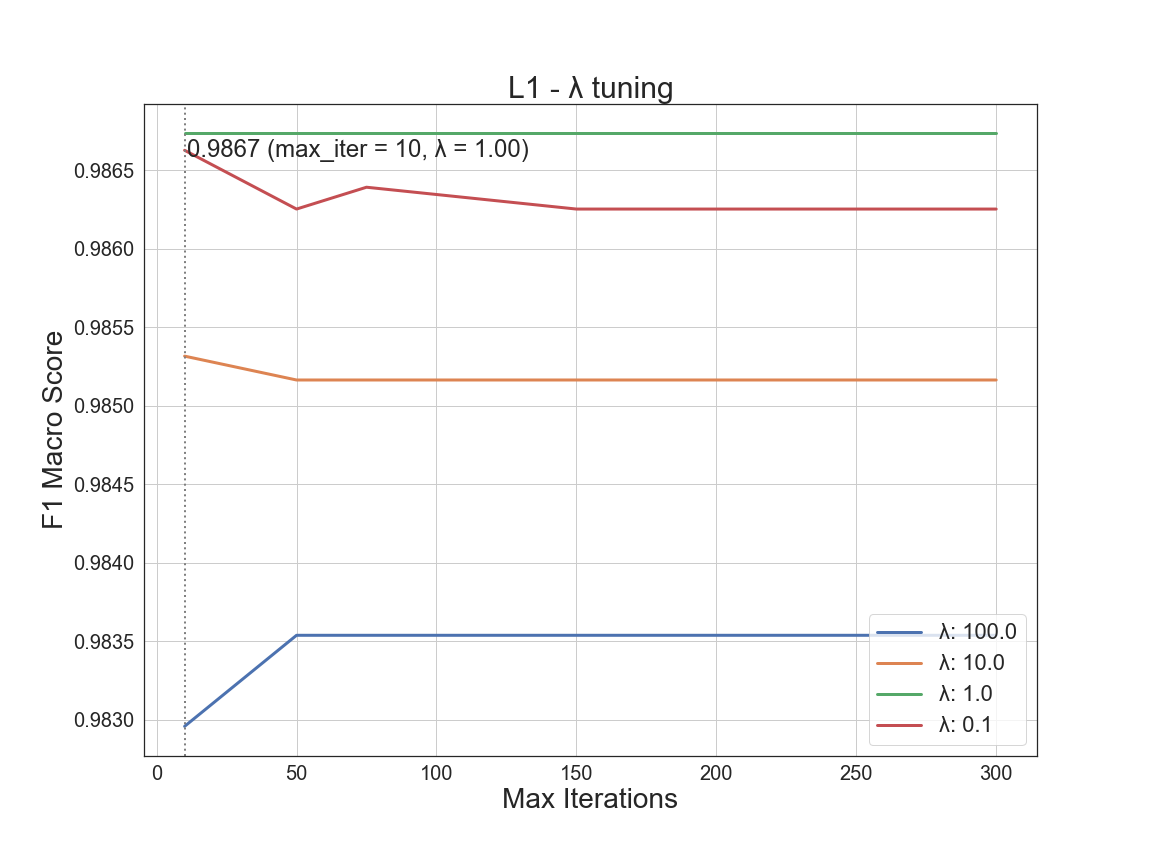
\includegraphics[width=\columnwidth]{chapter5/figure/logreg_l1_lambda.png}\par 
	\caption{Lasso, $ \lambda$ = [0.1, 1, 10, 100]}
	\label{fig:lr_lasso_lambda}
\end{figure}
\begin{figure}
	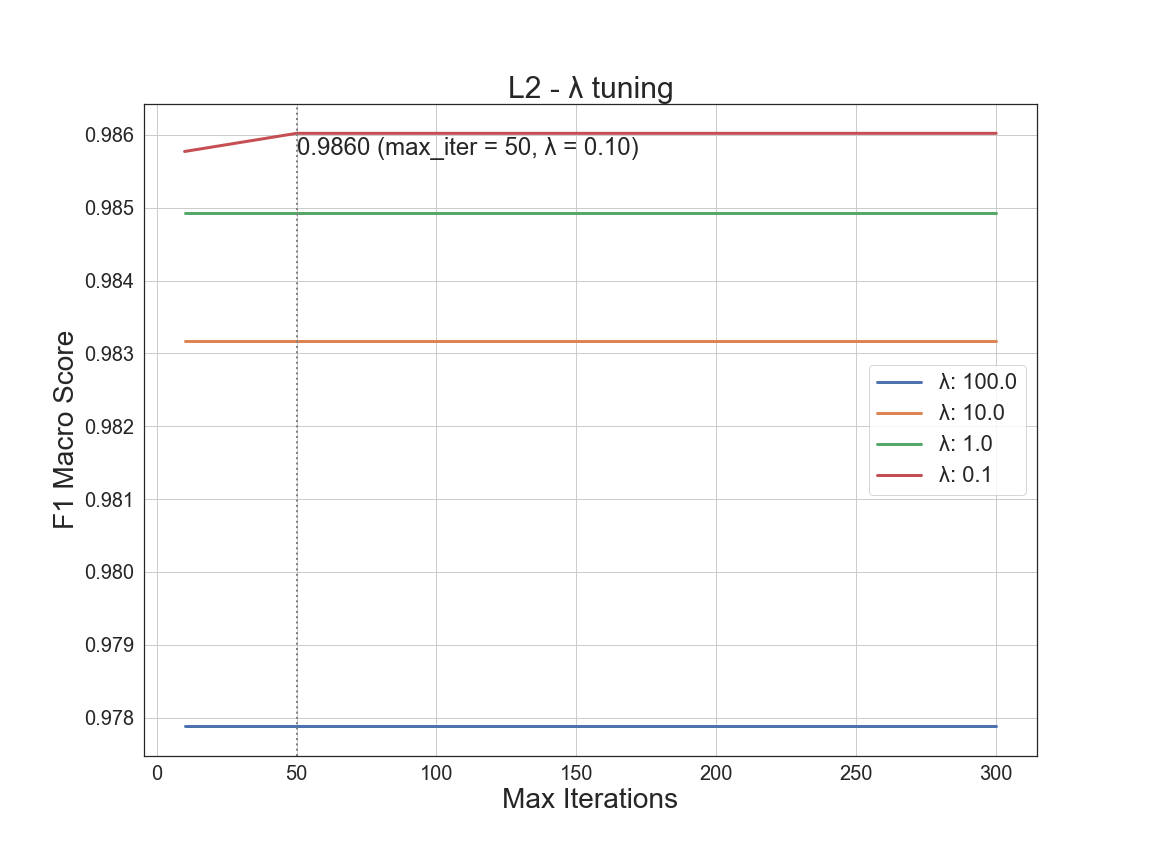
\includegraphics[width=\columnwidth]{chapter5/figure/logreg_l2_lambda.png}\par 
	\caption{Ridge, $ \lambda$ = [0.1, 1, 10, 100}
	\label{fig:lr_ridge_lambda}
\end{figure}

Figure \ref{fig:lr_lasso_lambda} highlights the slightly better results obtained with the Lasso penalty, with unitary $ \lambda $ coefficient (Lasso F1 score: 0.973).
The ridge penalty needs to be weakened ($ \lambda $ = 0.1) in order to top the Lasso performance, which is a compromise hard to deal with. The smaller the regularization coefficient, the higher the model complexity, as said before.
Moreover, we decided to gather further consideration, by looking inside the weighting applied by those two terms.

\begin{center}
	\begin{tabular}{@{}ccccc@{}}
		\multicolumn{5}{c}{\textbf{Ridge regularization}}\\
		\hline\hline
		\multicolumn{5}{c}{Binary Weights}\\
		\hline
		\multicolumn{1}{c|}{$ 5.1e^{-16} $}&
		\multicolumn{1}{c|}{$ 5.1e^{-16} $}&
		\multicolumn{1}{c|}{$ 5.1e^{-16} $}&
		\multicolumn{1}{c|}{$ 5.1e^{-16} $}&
		\multicolumn{1}{c}{$ -8.8e^{-17} $}\\
		\hline
		\multicolumn{5}{c}{Text-based Weights}\\
		\hline
		\multicolumn{1}{c|}{$ -2.2e^{-15} $}&
		\multicolumn{1}{c|}{$ -1.4e^{-14} $}&
		\multicolumn{1}{c|}{$ -5.1e^{-15} $}&
		\multicolumn{1}{c|}{$ -4.2e^{-15} $}&
		\multicolumn{1}{c}{$ 1.1e^{-16} $}\\
		\hline
		\multicolumn{5}{c}{Multiclass Weights}\\
		\hline
		\multicolumn{1}{c|}{$ -3.0e^{-15} $}&
		\multicolumn{1}{c|}{$ 2.0e^{-15} $}&
		\multicolumn{1}{c|}{$ -1.5e^{-16} $}&
		\multicolumn{1}{c|}{$ 5.7e^{-15} $}&
		\multicolumn{1}{c|}{$ -4.2e^{-15} $}\\
		\hline\hline\\
	\end{tabular}
\end{center}
The Ridge regularization leads to very small weights, and negative ones too. Even with unitary $ \lambda  $ coefficient, it is hard to distinguish a discrimination among features. This approach would have yielded a smoother model, but with the ability to give a chance to every classifier to distinguish among targets.
We wanted to get some further insights from the other weighting.

\begin{center}
	\begin{tabular}{@{}ccccc@{}}
		\multicolumn{5}{c}{\textbf{Lasso regularization}}\\
		\hline\hline
		\multicolumn{5}{c}{Binary Weights}\\
		\hline
		\multicolumn{1}{c|}{0.0}&
		\multicolumn{1}{c|}{0.0}&
		\multicolumn{1}{c|}{0.0}&
		\multicolumn{1}{c|}{0.0}&
		\multicolumn{1}{c}{1.391}\\
		\hline
		\multicolumn{5}{c}{Text-based Weights}\\
		\hline
		\multicolumn{1}{c|}{0.020}&
		\multicolumn{1}{c|}{1.297}&
		\multicolumn{1}{c|}{0.0}&
		\multicolumn{1}{c|}{0.182}&
		\multicolumn{1}{c}{0.952}\\
		\hline
		\multicolumn{5}{c}{Multiclass Weights}\\
		\hline
		\multicolumn{1}{c|}{1.316}&
		\multicolumn{1}{c|}{0.480}&
		\multicolumn{1}{c|}{1.457}&
		\multicolumn{1}{c|}{2.087}&
		\multicolumn{1}{c}{0.435}\\
		\hline\hline\\
	\end{tabular}
\end{center}
The L\textsubscript{1} term, as expected cut out some features from the model.
Looking at the excluded attributes, we noticed that the regularization caught the nature of the binary classifier. It wasn't supposed to give some contributes to the bots inner separation, its main purpose was to detect humans from content polluters.
Lasso seemed to understand this behaviour and decided to not consider the opinion of that classifier, when it comes to bot categories.
Another insight got from L\textsubscript{1} is about the treatment of the text-based classifier. the Naive Bayes model couldn't distinguish with certainty between NSFW and Spam-Bots, since they act in a similar way. They just tweets click-baiting links, with catchy captions. A "blind" classifier struggles in understand the nature of those links. This is the reason that almost two contributes of Naive Bayes had been discarded from the stacking model.

\begin{figure}
	\begin{multicols}{2}
		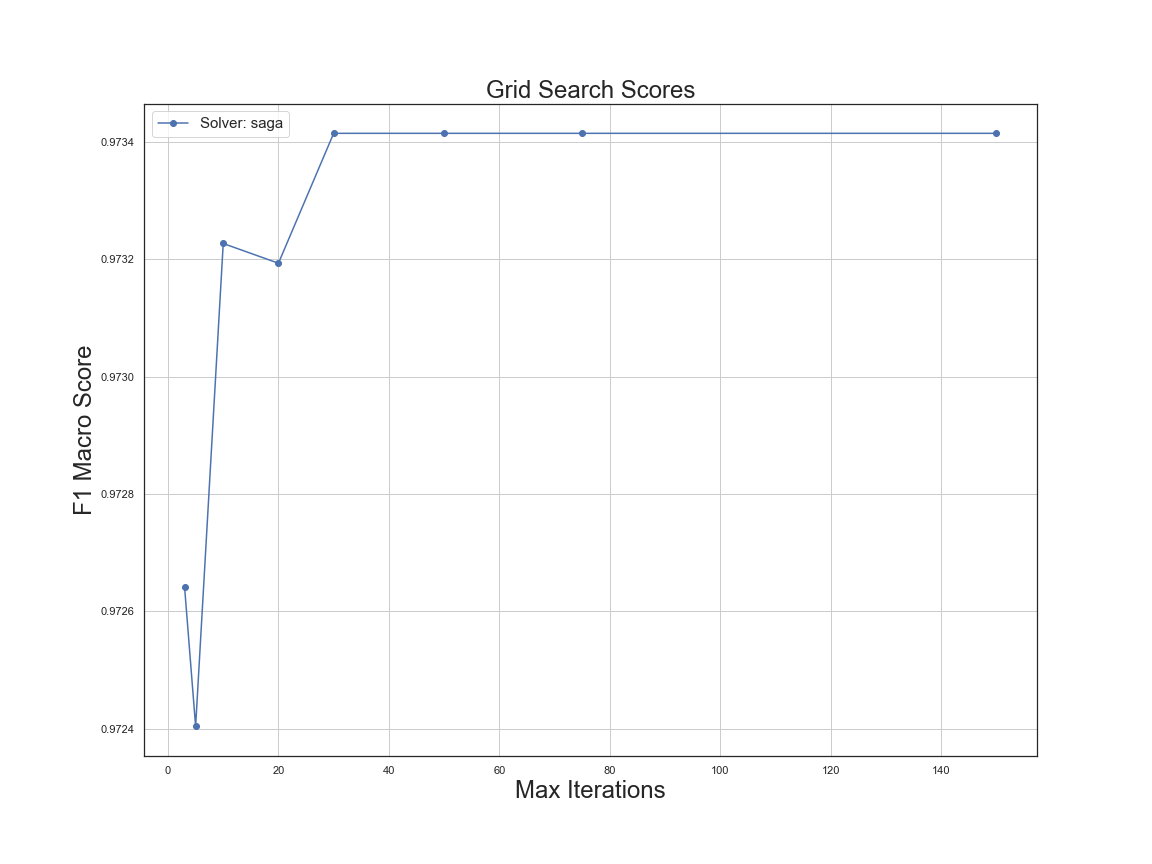
\includegraphics[width=\linewidth]{chapter5/figure/logreg_l1_close.png}\par 
		\caption{Up to 150 iterations}
		\label{fig:lr_lasso_close}
		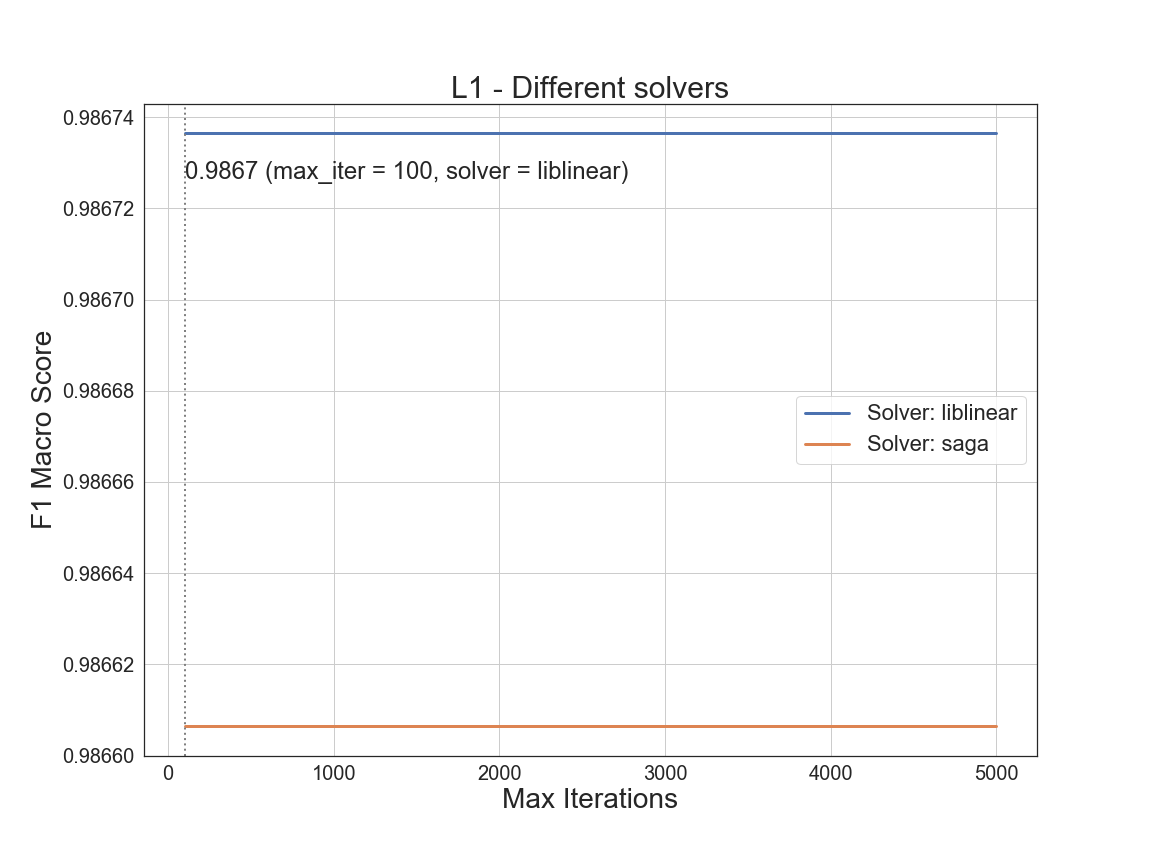
\includegraphics[width=\linewidth]{chapter5/figure/logreg_l1_far.png}\par 
		\caption{Up to 5000 iterations}
		\label{fig:lr_lasso_far}
	\end{multicols}
	\caption{Lasso Logistic Regression scores over solvers}
\end{figure}

Since we knew our dataset and we were aware of the bias it might contain, we preferred a lighter and sparser model, over a more complete one, even when the F1 scores used to match. We wanted our model to infer on new unseen data and to be ready to give a representative statistical description of the actual situation on Twitter.
We had to be far-sighted and not to recline on the accomplishments of the 10-fold crossvalidation. We thought that the Lasso model wuld had been performing better in out-of-box predictions.

We kept the L\textsubscript{1} penalty, with $ \lambda  = 1 $   and proceeded with the hyperparameters tuning.

Figure \ref{fig:lr_lasso_close} shows the trend in the F1 score, along with the increasing number of iterations, applying the \textit{SAGA}\cite{SAGA} solver (a variant of the \textit{Stochastic Average Gradient}\cite{SAG} optimization that supports Lasso penalty) and the \textit{LIBLINEAR}\cite{Liblinear}, an open source library for large-scale linear classification.

As it can be seen in Figures \ref{fig:lr_lasso_far}, by increasing the number of maximum iterations, up to 5000, the performances remain stable with every solver.
The algorithms seem to not improve after 75 maximum iterations setted.
Moreover, the SAGA solver gains slightly better results, in terms of F1 score, as it reaches 0.9734 in this metric, compared with the score obtained with LIBLINEAR solver, which is 0.9727.

The final Logistic Regression meta-classifier has been fitted with the Scikit-learn library, with this setting:\\
\textit{LogisticRegression(max\_iter = 100, penalty = "l1", solver = "saga", C = 1, multi\_class = "multinomial", fit\_intercept = True, class\_weight = "balanced")}.\\
The \textit{C} parameter stands for $ \frac{1}{\lambda} $, the regularization coefficient.
The balanced class weights means that the model automatically adjusts class weights inversely proportional to class frequencies in training set.\\
This setting obtained the following scores in a 10-fold crossvalidation:
\begin{itemize}
	\item[\PencilRight] \textit{Precision}: 0.972
	\item[\PencilRight] \textit{Recall}: 0.974
	\item[\PencilRight] \textit{F1 score}: 0.973
\end{itemize}
\section{Prediction pipeline}
\label{predicion_pipeline}
The final model is represented by a stacking ensemble with a defined execution pipeline for predictions.

As described by figure \ref{fig:prediction_pipeline}, In order to perform a prediction over a new sample the process is the following:
\begin{itemize}
	\item[\PencilRight]User and tweets data retrieving with Twitter APIs
	\item[\PencilRight]Prepare data and perform features engineering to output multiclass probability prediction (\textbf{Multiclass Random Forest})
	\item[\PencilRight]Prepare data and strip multiclass features to output binary probability prediction (\textbf{Binary Random Forest})
	\item[\PencilRight]Prepare and treat text to perform text-based probability prediction (\textbf{Text-based Naive Bayes})
	\item[\PencilRight]Build new features vector with the stacked outcomes of the previous classifiers
	\item[\PencilRight]Compute the final mutliclass probabilistic prediction with the meta-classifier (\textbf{Multinomial Logistic Regression})
\end{itemize}
The produced probability vector assesses the nature of the examined user.
It will be handled by a web application, in order to provide a useful classification tool for every internet user.
The engine of this web application is mainly composed by a python script, which, given a Twitter user name, resumes this prediction pipeline and executes it, providing the classification.

This last lines anticipate the content of the following chapter of our thesis.
\begin{figure}
	\begin{center}
		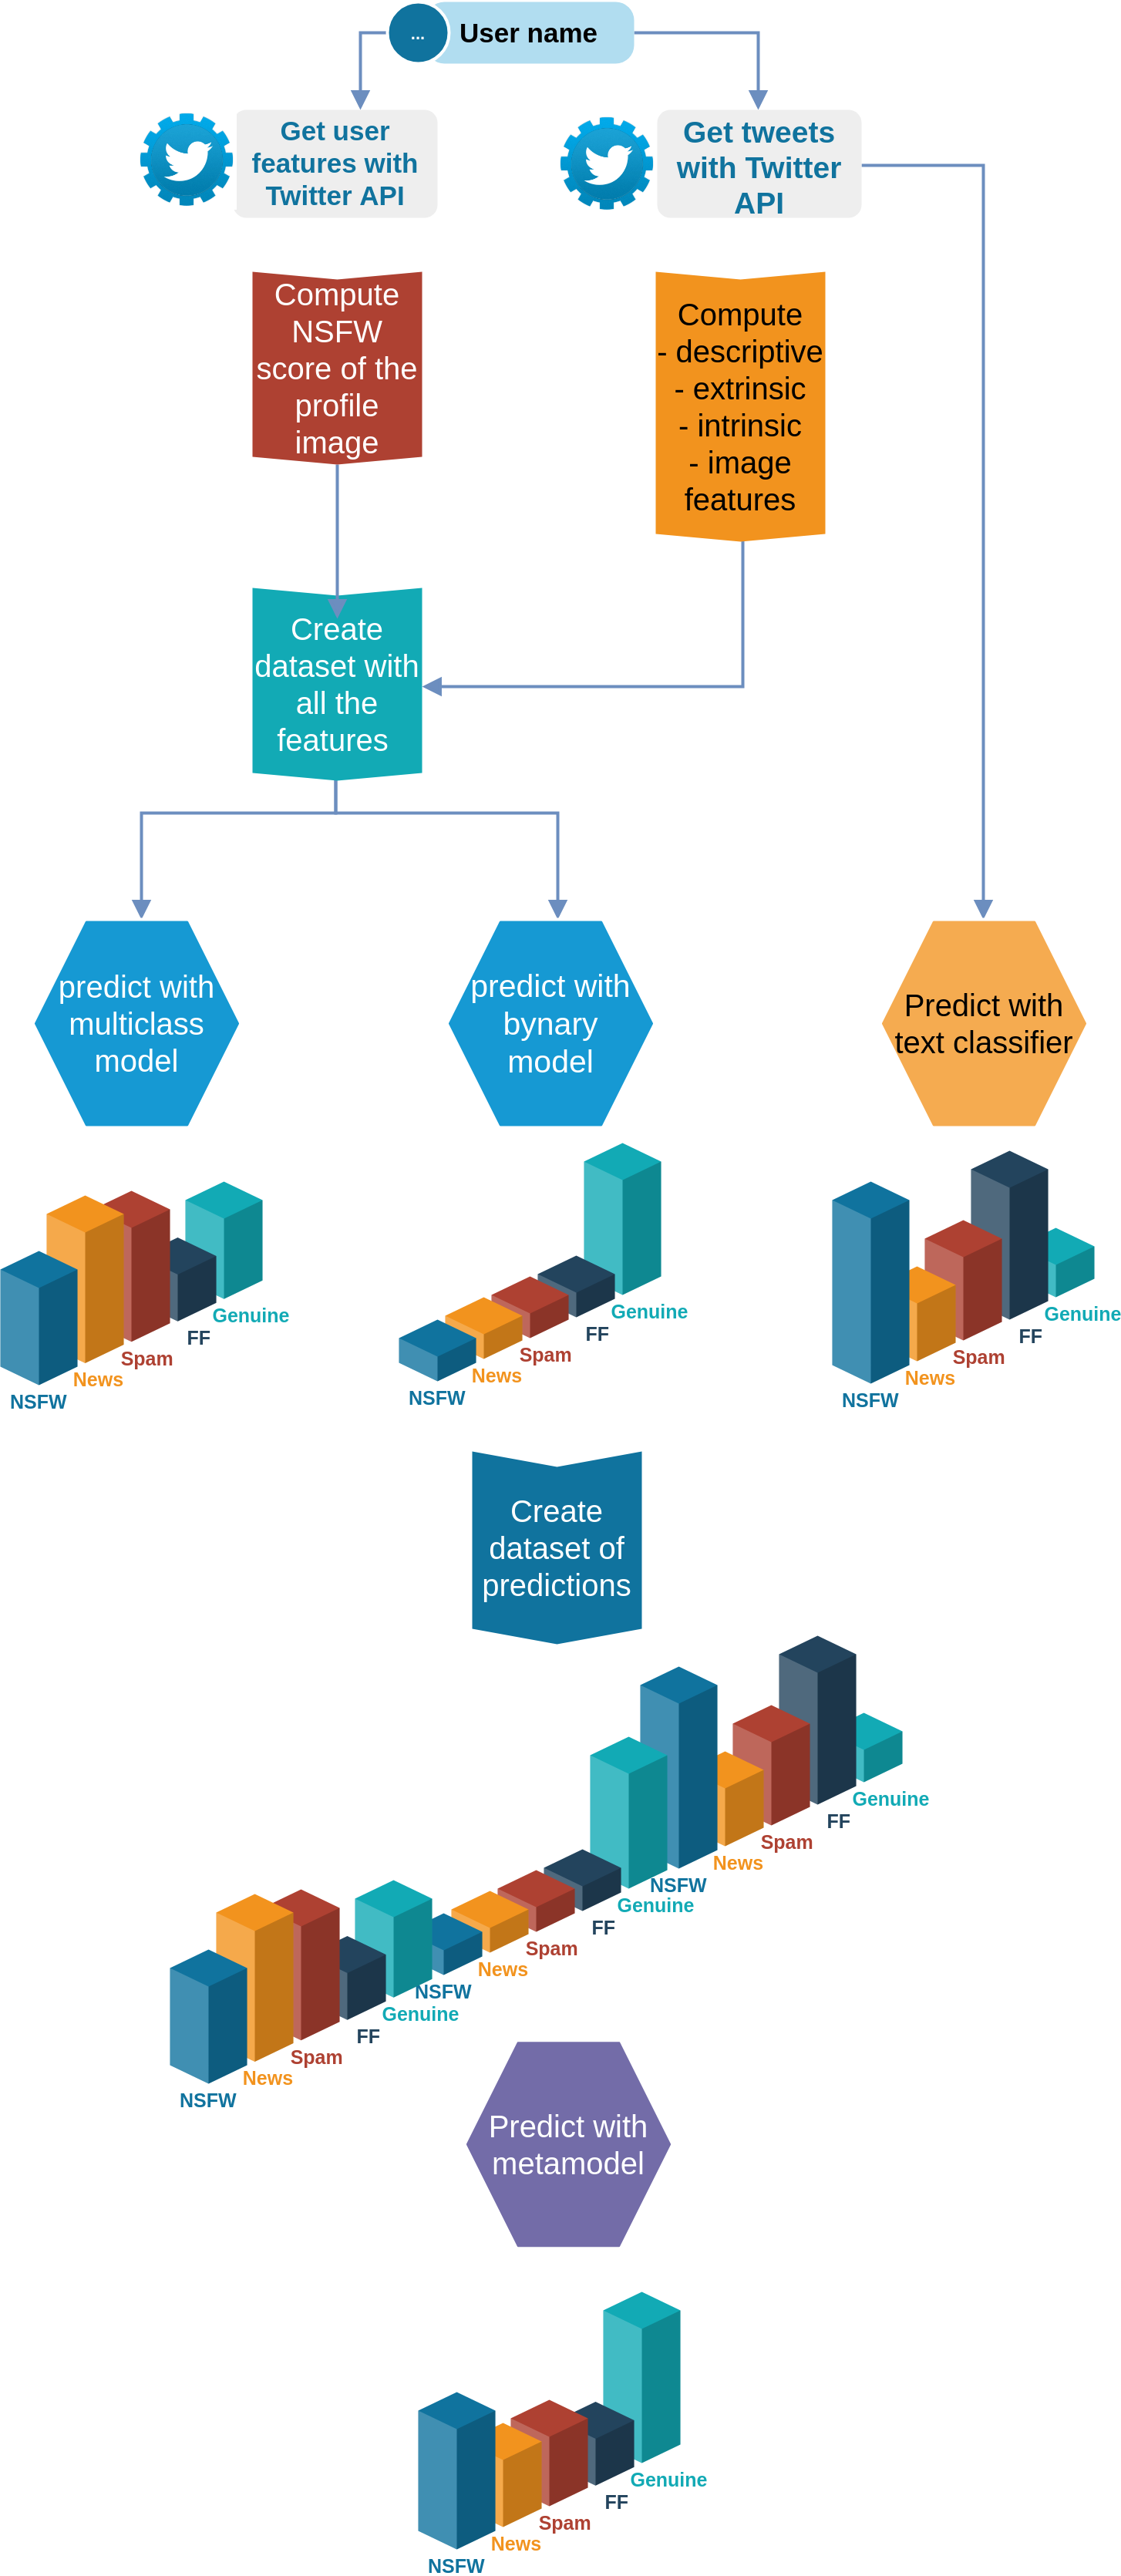
\includegraphics[width=0.8\columnwidth]{chapter5/figure/prediction.png}\par 
	\end{center}
	\caption{Final prediction pipeline}
	\label{fig:prediction_pipeline}
\end{figure}